%% =====================================================================
%%  Journal version — CMPB (Elsevier) submission.
%%  Class: elsarticle, review option (double-spaced), 12pt.
%%  Target: Computer Methods and Programs in Biomedicine.
%% =====================================================================
\documentclass[review,12pt]{elsarticle}

\usepackage[T1]{fontenc}
\usepackage[utf8]{inputenc}
\usepackage{amsmath,amssymb}
\usepackage{graphicx}
\usepackage{booktabs}
\usepackage{array}
\usepackage{multirow}
\usepackage{threeparttable}
\usepackage[font=small,labelfont=bf,skip=6pt]{caption}
\usepackage{subcaption}
\usepackage{enumitem}
\usepackage{microtype}
\usepackage{xcolor}
\usepackage{orcidlink}
\usepackage{url}

\setlist[itemize]{topsep=2pt,itemsep=1pt,parsep=0pt,leftmargin=1.4em}
\setlist[enumerate]{topsep=2pt,itemsep=1pt,parsep=0pt,leftmargin=1.6em}
\renewcommand{\arraystretch}{1.12}

% Let floats sit near their first mention instead of drifting to the end.
\renewcommand{\topfraction}{0.95}
\renewcommand{\bottomfraction}{0.9}
\renewcommand{\textfraction}{0.05}
\renewcommand{\floatpagefraction}{0.7}
\setcounter{topnumber}{4}
\setcounter{bottomnumber}{2}
\setcounter{totalnumber}{6}

\journal{Computer Methods and Programs in Biomedicine}

\begin{document}

\begin{frontmatter}

\title{Reproducible Evaluation of Breast Cancer Classifiers: Protocol Validation, Feature-Selection Stability, and Multi-Method Interpretation}

\author[inst1]{Jeremiah Masaba\corref{cor1}\orcidlink{0009-0004-5620-996X}}
\ead{jericho555@yahoo.com}
\cortext[cor1]{Corresponding author. Tel.: +256\,702\,920\,266; E-mail: jericho555@yahoo.com}
\address[inst1]{Department of Computer Science, School of Computing and Informatics Technology, Makerere University, Kampala, Uganda, P.O. Box 7061}

\begin{abstract}
\textbf{Background and Objective:} Fine-needle aspiration (FNA) of a breast mass yields a short vector of nuclear measurements, and the Wisconsin Diagnostic Breast Cancer (WDBC) dataset is the standard tabular benchmark for separating benign from malignant samples. Reported accuracies sit near the ceiling that 569 samples can resolve, so the paper asks whether a reduced feature set preserves accuracy across a wide model comparison, whether the resulting decision can be explained by several independent methods, and whether the protocol is reproducible.
\textbf{Methods:} Twenty-five model configurations, spanning 20 distinct learning algorithms (linear models, tree-based ensembles, support vector machines, instance-based and probabilistic models, neural networks and stacking ensembles), were compared on WDBC at native and standardised scale, with all 30 features and with a 12-feature recursive feature elimination (RFE) subset. The protocol includes stratified repeated cross-validation (5-fold $\times$ 4 repeats = 20 folds) with the selector fitted inside each fold, nested hyperparameter tuning, an RFE-$k$ sweep from $k=4$ to $k=30$, multi-method interpretation (SHAP with interaction values, permutation importance, logistic coefficients, partial dependence, LIME stability), and model agreement analysis across five ensemble variants.
\textbf{Results:} A stacking ensemble with logistic meta-learner classified 141 of 143 held-out samples correctly (AUC 0.9973, Brier 0.0180), matching logistic regression L2 on standardised RFE-12 features (AUC 0.9988); stochastic gradient descent reached the highest AUC (0.9990). Across twenty stratified folds the reduction from 30 to 12 features was indistinguishable (paired $p=0.400$), while standardisation improved logistic regression significantly (paired $p<0.001$). Interpretation converged on concave points mean and worst-case texture as the leading predictors, with worst-case area and perimeter close behind, and 30.4\% of the prediction mass on feature pairs rather than main effects. The models agreed on 136 of 143 cases, with one genuinely hard case missed by all.
\textbf{Conclusions:} The comparison, protocol validation and interpretation suite provide a template for reproducible classifier evaluation on small clinical datasets, and show that the retained feature subset is one draw from a redundant family rather than a unique clinical finding.
\end{abstract}

\begin{keyword}
Breast cancer diagnosis \sep Recursive feature elimination \sep Classifier comparison \sep Stratified cross-validation \sep Explainable machine learning \sep Model agreement
\end{keyword}

\end{frontmatter}

\section{Introduction}

Breast cancer is the most frequently diagnosed cancer among women and accounts for close to one third of new female cancer cases \cite{wilkinson2022understanding,kashyap2022global}. Outcomes depend on the stage at which the disease is found, so a reliable, cheap and reproducible triage of a suspicious mass has clinical value \cite{katsura2022breast}. Fine-needle aspiration (FNA) is the least invasive sampling route, and in the digitised workflow behind the data studied here a computerised scan of the aspirate returns a vector of nuclear measurements whose reported interpretation accuracy varies widely between sites \cite{alkuwari2008accuracy}, which is the usual argument for pairing the vector with a classifier. The Wisconsin breast cancer datasets have been the standard tabular testbed for this task since the 1990s \cite{street1993nuclear}; two versions are routinely conflated: the original dataset (WBCD, 699 samples, 9 integer features) and the diagnostic set (WDBC, 569 samples, 30 continuous features from 10 nuclear descriptors). Several widely cited comparisons use the first \cite{salama2012experimental,lavanya2011analysis,hazra2016study,wang2018support}; this study uses the second (Section~\ref{sec:related}).

Because 143 test cases cannot separate models that differ by one or two cases, and because rankings are confounded by protocol details often left unreported (the split, whether feature selection saw the test partition, which hyperparameters were tuned), this paper asks five questions. (RQ1) Does recursive feature elimination (RFE) change classifier accuracy on WDBC, and by how many samples, across a 25-model comparison? (RQ2) Is the retained subset stable when the partition changes, or when one partition is fitted twice? (RQ3) Which measurements survive elimination, and do they form a coherent clinical story? (RQ4) Do SHAP, permutation importance, partial dependence, logistic coefficients and LIME agree with the retained set? (RQ5) Does a stratified cross-validation protocol with the selector inside each fold confirm the single-partition results?

The contributions are:
\begin{itemize}
\item a comparison of 25 model configurations (20 distinct learning algorithms) on both native and standardised scales, with RFE-12 and full-30 features, reported as counts of correctly classified samples with confusion matrices, AUC, Brier score and interval estimates, plus the protocol needed to reproduce it;
\item a stratified repeated cross-validation protocol (20 folds) with the selector fitted inside each fold, plus nested hyperparameter tuning, addressing the reproducibility gaps identified in prior work;
\item a paired comparison of the full and reduced model across thirty partitions, and a stability analysis of the retained subset across partitions and repeated fits of one partition;
\item multi-method post-hoc explanations (SHAP with interaction values, permutation importance, partial dependence, logistic coefficients, LIME stability) read against the set that RFE retained, and a model agreement analysis across five ensemble variants;
\end{itemize}

The contribution sits in three structural claims rather than in a headline score, which the data cannot resolve. First, the feature selector is treated as part of the pipeline and refitted inside every held-out fold rather than once at the start. Second, the retained subset is a partition artefact drawn from a redundant family of near-equivalent twelve-feature sets: it changes under resampling and again under a numerical-library upgrade, so it is not a fixed clinical finding. Third, an agreement-plus-interpretation suite quantifies the genuinely hard cases (case 82, missed by all five ensembles) instead of averaging them away. Together these turn a ceiling accuracy into a statement about what WDBC can and cannot support, and the answer is narrower than the published literature implies.

%% =====================================================================
\section{Related Work}
\label{sec:related}

Classical comparisons on the Wisconsin data report accuracies between roughly 94\% and 98\%. Salama et al.\ led an SMO support vector machine at 97.0\% across three datasets \cite{salama2012experimental}; Lavanya and Rani reached 95.1\% with six attributes retained \cite{lavanya2011analysis}; further comparisons of naive Bayes, SVM and ensemble learners appear in \cite{hazra2016study,wang2018support,durgalakshmi2020feature,bah2022analysis}. Yildirim reported 98.2\% on WDBC with a wavelet-PCA-SVM pipeline in this journal \cite{yildirim2015hybrid}. Several of these studies use the 699-sample WBCD rather than the 569-sample WDBC studied here, and their protocols differ in ways that are often left unreported (split rule, selector scope, hyperparameter grid), so cross-paper rankings are indicative at best.

A second line of work has moved off the compact FNA vector: multitask networks on mammographic imaging \cite{shi2022emtn}, deep features learned from whole-slide tiles \cite{lee2020unsupervised}, semi-supervised survival prediction on longitudinal follow-up \cite{hassanzadeh2015semi}. Each requires an input an FNA workflow does not produce, which keeps the 30-feature vector the relevant target for the aspiration-cytology setting this paper addresses.

The methodological critique this paper engages with concerns evaluation protocols. Kaufman et al.\ formalised target-dependent leakage in data mining and catalogued how feature selection, imputation and resampling each introduce it \cite{kaufman2012leakage}. Kapoor and Narayanan documented leakage across published clinical-ML claims and, in the specific case of the Wisconsin data, reported that several published accuracies do not survive a corrected protocol \cite{kapoor2023leakage}. Their remedy is standard: wrap the preprocessor and the selector as the first stage of a pipeline that is refitted inside every held-out fold. The classical WDBC literature largely predates this convention.

Two further bodies of work qualify what a retained subset and its post-hoc explanations can bear. Nogueira et al.\ quantified feature-selection stability across dozens of datasets and showed that even a fixed selector returns substantially different subsets under resampling, so a specific retained list is rarely reproducible enough to carry a clinical claim \cite{nogueira2018stability}. On the interpretation side, Arrieta et al.\ surveyed the requirements XAI must meet for high-stakes reasoning \cite{arrieta2020xaiconcept}, and Rudin argued that in medical settings post-hoc explanations of opaque models can be misleading and that interpretable models should be preferred where feasible \cite{rudin2019stop}. This paper reads that critique seriously: alongside the XGBoost model it explains, it reports a standardised logistic regression on the same twelve features as an inherently interpretable second view.

On the method side, RFE \cite{guyon2002rfe} reduces a feature space by iteratively dropping the weakest predictor, while SHAP \cite{lundberg2017shap}, LIME \cite{ribeiro2016lime}, permutation importance \cite{altmann2010universal} and partial dependence \cite{friedman2001greedy} describe a fitted model, and the accountability literature argues that transparency should be evidenced rather than asserted \cite{gianfagna2021xai,narayanan2007ai}. The two strands rarely meet on tabular clinical data: selection ablations are reported without explanations, and explanation studies rarely ablate the feature set behind the explained model. What is missing is a WDBC study that reports a classifier comparison at the granularity the data support, isolates the effect of a feature subset, checks multiple explanations against the retained subset, and states a reproducible protocol; this paper supplies it.

%% =====================================================================
\section{Materials and Methods}
\label{sec:method}

\subsection{Dataset}

WDBC describes 569 FNA samples (357 benign, 212 malignant), each summarised by 30 continuous features \cite{street1993nuclear,kaggle2016wdbc}: ten nuclear descriptors (radius, texture, perimeter, area, smoothness, compactness, concavity, concave points, symmetry, fractal dimension), each reported as a mean, a standard error and a worst (largest) value. The dataset is public and contains no personally identifying information; it predates this study.

\subsection{Preprocessing}

The identifier and trailing unnamed columns were discarded and the diagnosis encoded as a binary label (benign 0, malignant 1); no value required imputation. Two arms were tested: native scale (no transformation), and standardised scale (zero mean, unit variance fitted on training rows only). Figure~\ref{fig:pipeline} summarises the pipeline.

\begin{figure}[ht!]
\centering
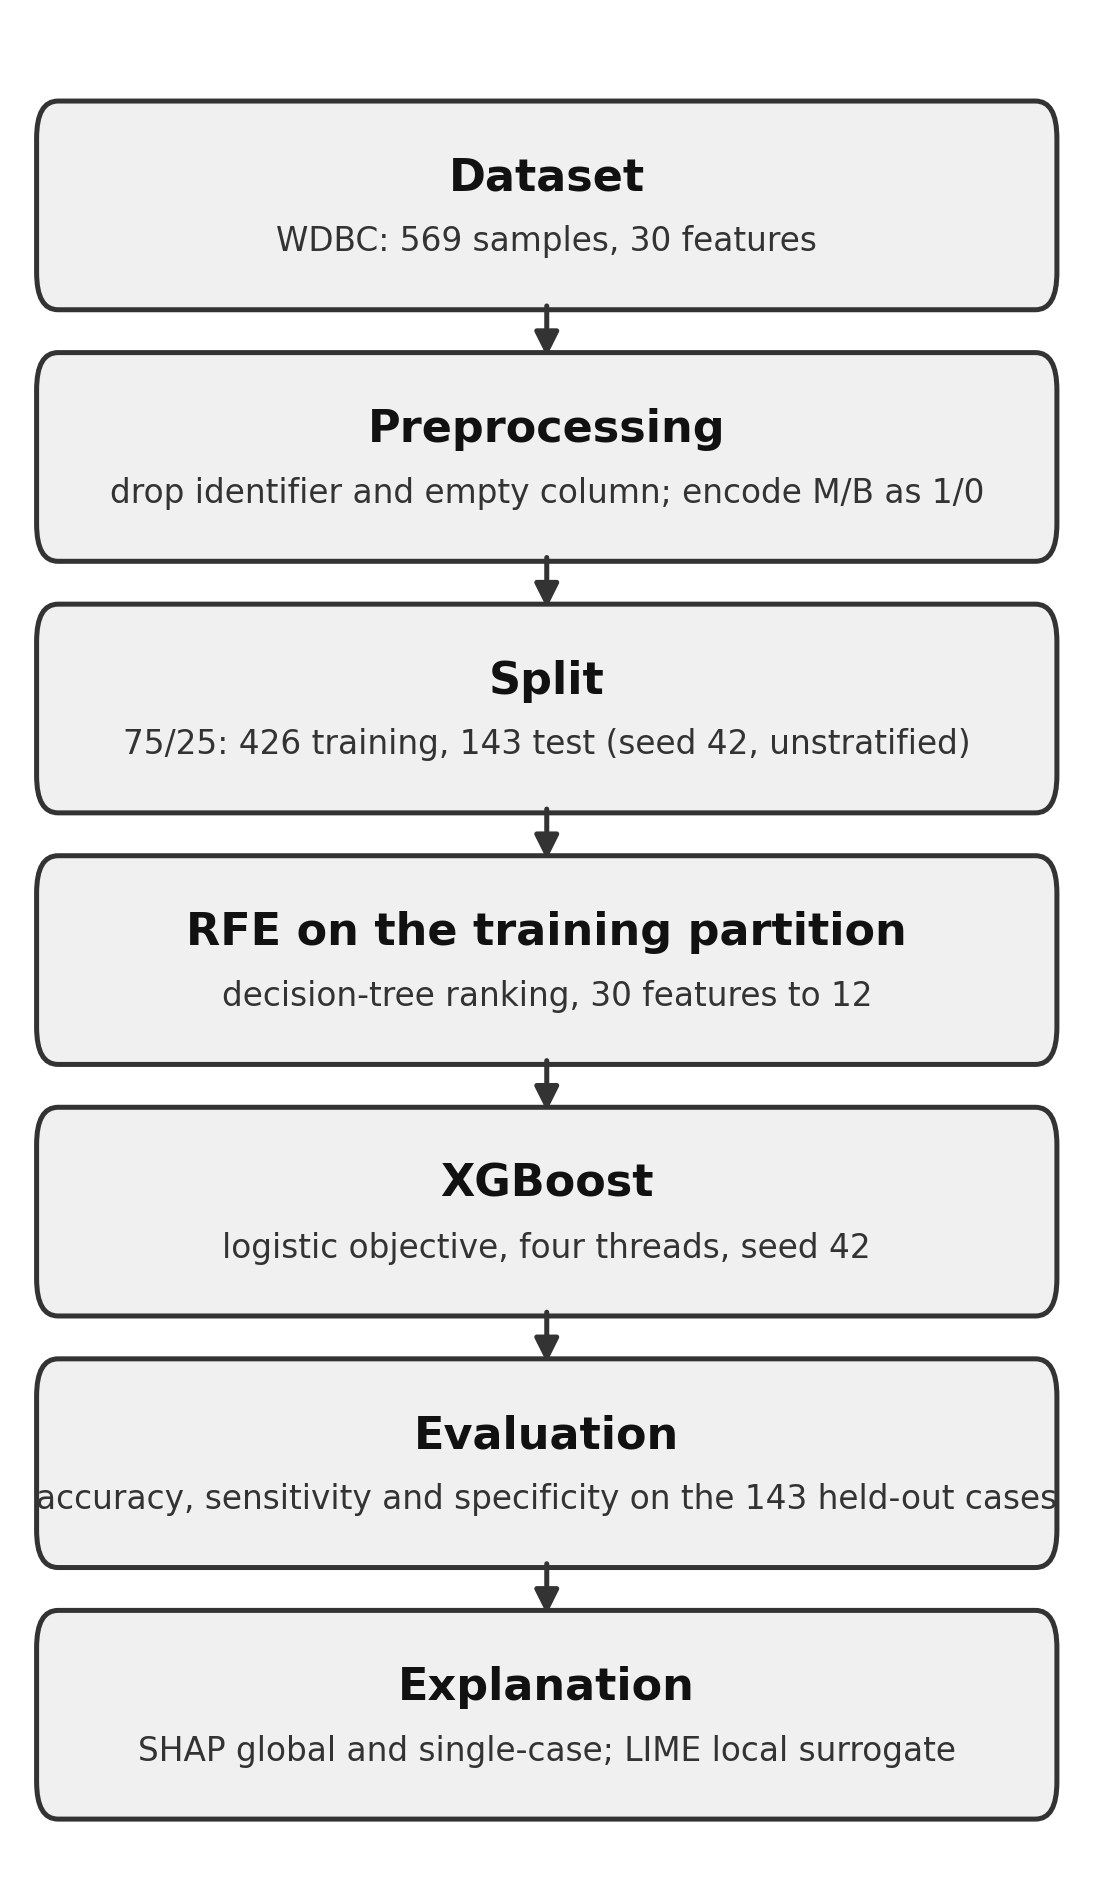
\includegraphics[width=0.85\textwidth]{figures/fig_pipeline.png}
\caption{Complete analytical pipeline. The dataset is split 75/25 (426 training, 143 test). Two preprocessing arms (native, standardised) are each evaluated with full-30 and RFE-12 features across 25 model configurations. The interpretation suite applies SHAP, permutation importance, logistic coefficients, partial dependence, and LIME stability to the highest-performing configurations. Protocol validation uses stratified 20-fold CV with the selector inside each fold, nested hyperparameter tuning, and an RFE-$k$ sweep.}
\label{fig:pipeline}
\end{figure}

\subsection{Classifiers and settings}

Twenty-five model configurations, spanning 20 distinct learning algorithms from seven families, were trained with scikit-learn \cite{pedregosa2011scikit}, with the boosted ensemble supplied by xgboost 1.7.2 \cite{chen2016xgboost} on numpy 1.26.4: linear models (logistic regression with L2, L1 and elastic-net penalties; ridge \cite{hoerl1970ridge}; SGD with log loss \cite{shalev2011pegasos}; LDA; QDA; nearest centroid); tree-based ensembles (random forest \cite{breiman2001random}, extra trees \cite{geurts2006extremely}, gradient boosting \cite{friedman2001greedy}, AdaBoost \cite{freund2012short}, XGBoost, histogram-based gradient boosting \cite{ke2017lightgbm}, bagging); support vector machines (linear \cite{cortes1995support}, RBF, Nu-SVC \cite{scholkopf2000new}); K-nearest neighbours ($k=20$); a multilayer perceptron (one hidden layer of 100 rectified-linear units, Adam, $\alpha=10^{-4}$, default and seeded configurations); a Gaussian process classifier \cite{rasmussen2006gaussian}; and meta-estimators (soft and hard voting; stacking of random forest and XGBoost with a logistic meta-learner) \cite{wolpert1992stacked}. All values except $k$ and the stacking meta-learner are library defaults; each arm was evaluated with all 30 features and with RFE-12 (full configuration list in the accompanying repository).

\subsection{Recursive feature elimination}

RFE fits an estimator, ranks predictors by their importance to it, drops the weakest and repeats until a stopping rule is met \cite{guyon2002rfe}. The wrapper here was a single decision tree at library defaults, removing one predictor at a time to a fixed count of 12, set as a design constant rather than tuned by cross-validation in the reference pipeline; twelve sits between the very-small subsets typical of prior WDBC work (6 attributes in \cite{lavanya2011analysis}) and the 15--20 a loose sample-size heuristic would allow at 426 training rows, and the RFE-$k$ sweep (Section~\ref{sec:protocol}) confirms 12 is at the accuracy peak. The selector was the first pipeline stage, fitted on the 426 training samples only; the 143 test samples never saw it, the arrangement the method requires and one easily broken by fitting the selector on the full dataset. An unseeded wrapper tree returns a different fit on identical rows, so it was seeded (\texttt{random\_state=0}); Section~\ref{sec:elim} reports both the seeded result and the unseeded spread.

\subsection{Split, metrics and granularity}

The dataset was divided 75/25 with a fixed seed of 42: 426 training samples, 143 test samples (89 benign, 54 malignant). The partition was shuffled but not stratified; at this prevalence the draw preserved the class balance to within one percentage point. Because 143 cases cannot separate models that differ by one or two cases, the full-versus-reduced comparison was repeated over thirty partitions (seeds 0--29) with the selector seeded as above, so every result can be regenerated.

Accuracy, precision, recall and specificity are reported with the confusion matrix, because for a diagnostic aid the false-negative count matters more than the accuracy; AUC, Brier score, log-loss and expected calibration error (ECE) are reported where the model emits probabilities. Wilson intervals at $n=143$ span about five percentage points at 140/143 (94.0--99.3\%) and widen as accuracy falls.

\subsection{Post-hoc explanation}

Two reference models were explained rather than one. M\_REF is the unscaled XGBoost fit on RFE-12 (140/143), chosen because TreeSHAP is exact on boosted trees and because this is what the reference stack produces; the choice is protocol-driven, not accuracy-driven (SGD at AUC 0.9990, stacking and logistic L2 at 141/143 all outscore it). M\_LIN is the standardised logistic regression on the same twelve features (141/143), the inherently interpretable counterpart the explanation literature asks for \cite{rudin2019stop}. Five methods were then applied. (1) TreeSHAP \cite{lundberg2017shap} attributions with interaction values on the 143 test cases of M\_REF. (2) M\_LIN logistic coefficients exponentiated to odds ratios with 95\% Wald intervals. (3) Permutation importance \cite{altmann2010universal} for four families (XGBoost, random forest, extra trees, standardised logistic L2): each of the twelve columns shuffled in isolation over 50 seeded repeats, recording the mean accuracy drop and its standard deviation. (4) Partial dependence plots \cite{friedman2001greedy} for the top four features. (5) LIME \cite{ribeiro2016lime} stability over five seeds for 12 malignant cases, scored by the Jaccard index of the top-5 features.

\subsection{Protocol validation}
\label{sec:protocol}

Three protocol validations: (1) \textbf{Stratified repeated CV}: 5-fold $\times$ 4 repeats (20 folds) with RFE fitted inside each training fold, so the held-out fold never influenced the subset, across nine configurations spanning XGBoost, logistic regression, random forest, SVM and MLP at both scales and feature sets; (2) \textbf{Nested hyperparameter tuning}: GridSearchCV with 3-fold inner CV nested inside the outer 5-fold CV for SVM, logistic regression and MLP, nothing selected on the outer test fold; (3) \textbf{RFE-$k$ sweep}: $k$ from 4 to 30 with 20 stratified folds per $k$, testing whether 12 is near-optimal.

\subsection{Model agreement analysis}

Five models fitted on standardised RFE-12 tested whether the highest-scoring configurations agree case-by-case. The set was chosen to span five different families among those scoring 138/143 or above on the reference partition: histogram gradient boosting and SGD (boosting and stochastic-gradient linear), bagging (a bootstrap ensemble), ridge (a linear classifier) and stacking (a meta-estimator). Two top performers were left out by family overlap: logistic regression L2, on the same linear side as ridge, and XGBoost, on the same boosting side as histogram gradient boosting. Agreement is the fraction of the 143 cases on which a pair predicts the same label; majority vote requires three of five, and disagreement cases are described in standard deviations from the cohort mean.

%% =====================================================================
\section{Results and Discussion}
\label{sec:results}

\subsection{Structure of the data}
\label{sec:struct}

Figure~\ref{fig:eda} summarises the exploratory data analysis: the 569 samples comprise 357 benign (62.7\%) and 212 malignant (37.3\%) cases, the PCA projection separates the two classes in the first two components with PC1 (dominated by size features) capturing 43.7\% of the variance, and 21 of the 435 feature pairs correlate at $|r|\ge 0.9$.

\begin{figure}[ht!]
\centering
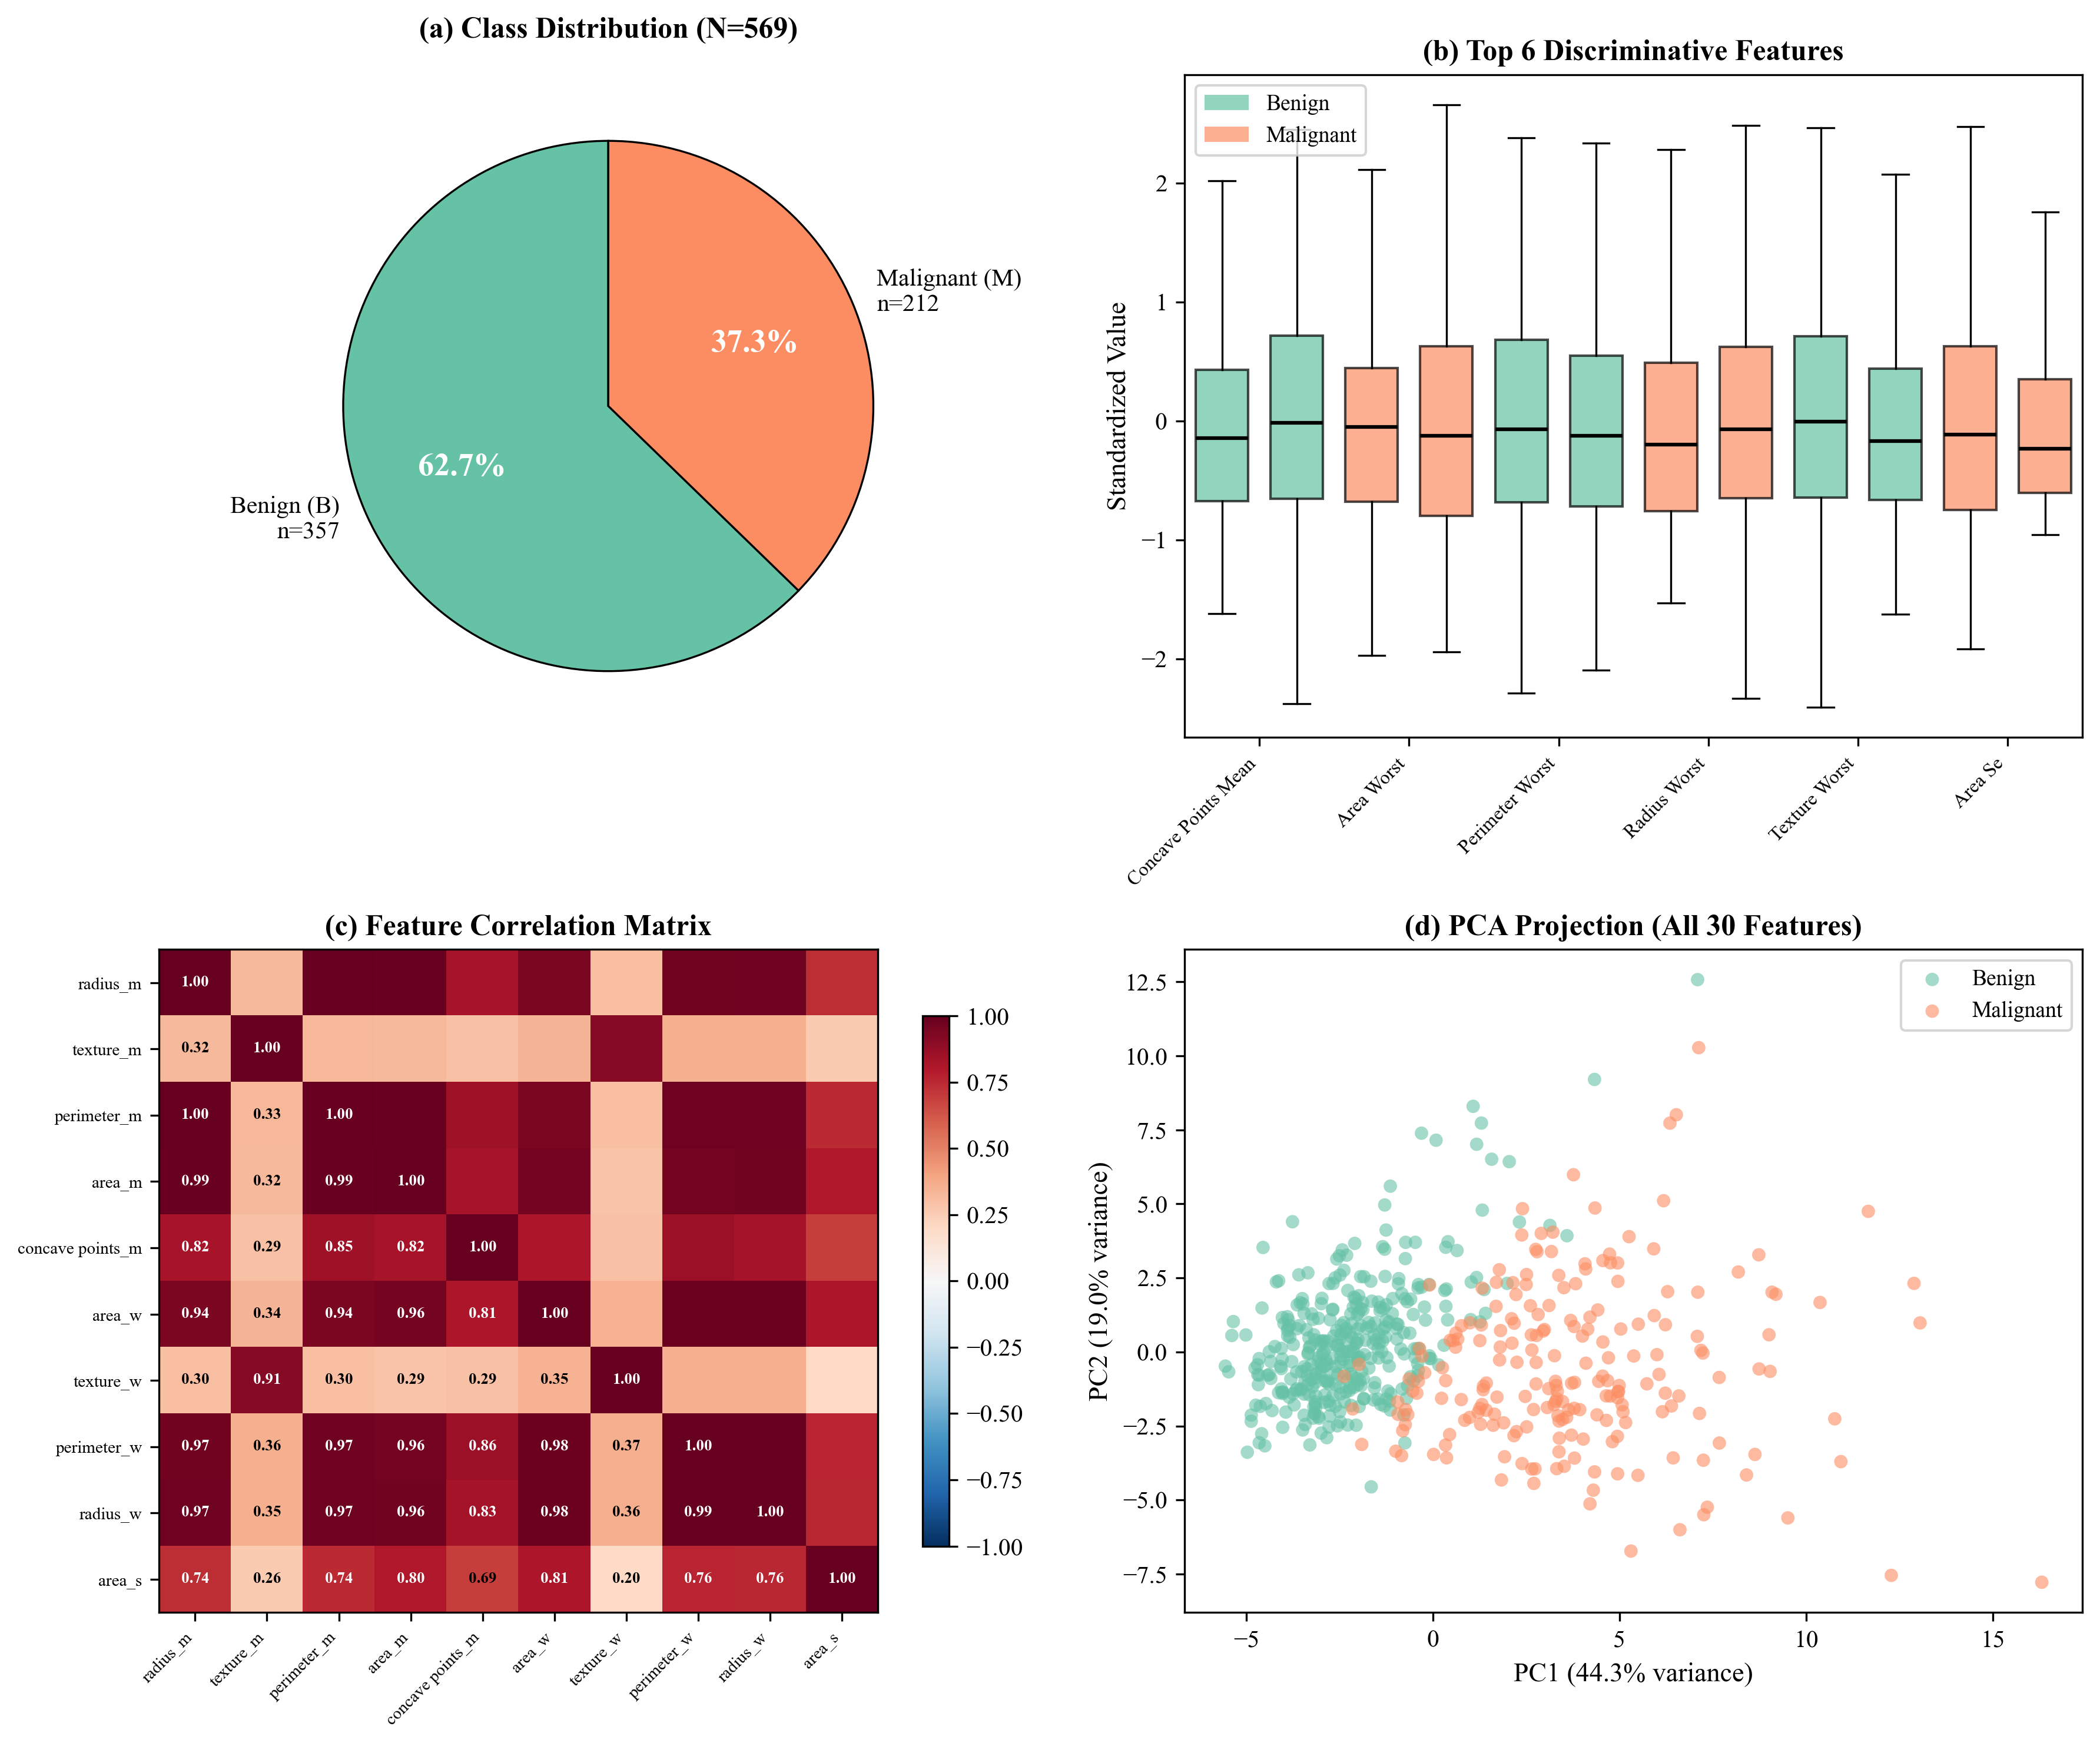
\includegraphics[width=\textwidth]{figures/fig_eda_overview.png}
\caption{Exploratory data analysis overview. (a) Class distribution: 357 benign vs.\ 212 malignant samples. (b) Top 6 discriminative features shown as standardised box plots by diagnosis. (c) Pearson correlation matrix of 10 key features; radius/area/perimeter features are highly inter-correlated ($|r|>0.9$). (d) PCA projection of all 30 standardised features showing clear class separation.}
\label{fig:eda}
\end{figure}

Figure~\ref{fig:distributions} shows the six most discriminative features by class: separation is clearest for concave points mean, area worst and perimeter worst, consistent with malignant nuclei being larger and more irregular.

\begin{figure}[ht!]
\centering
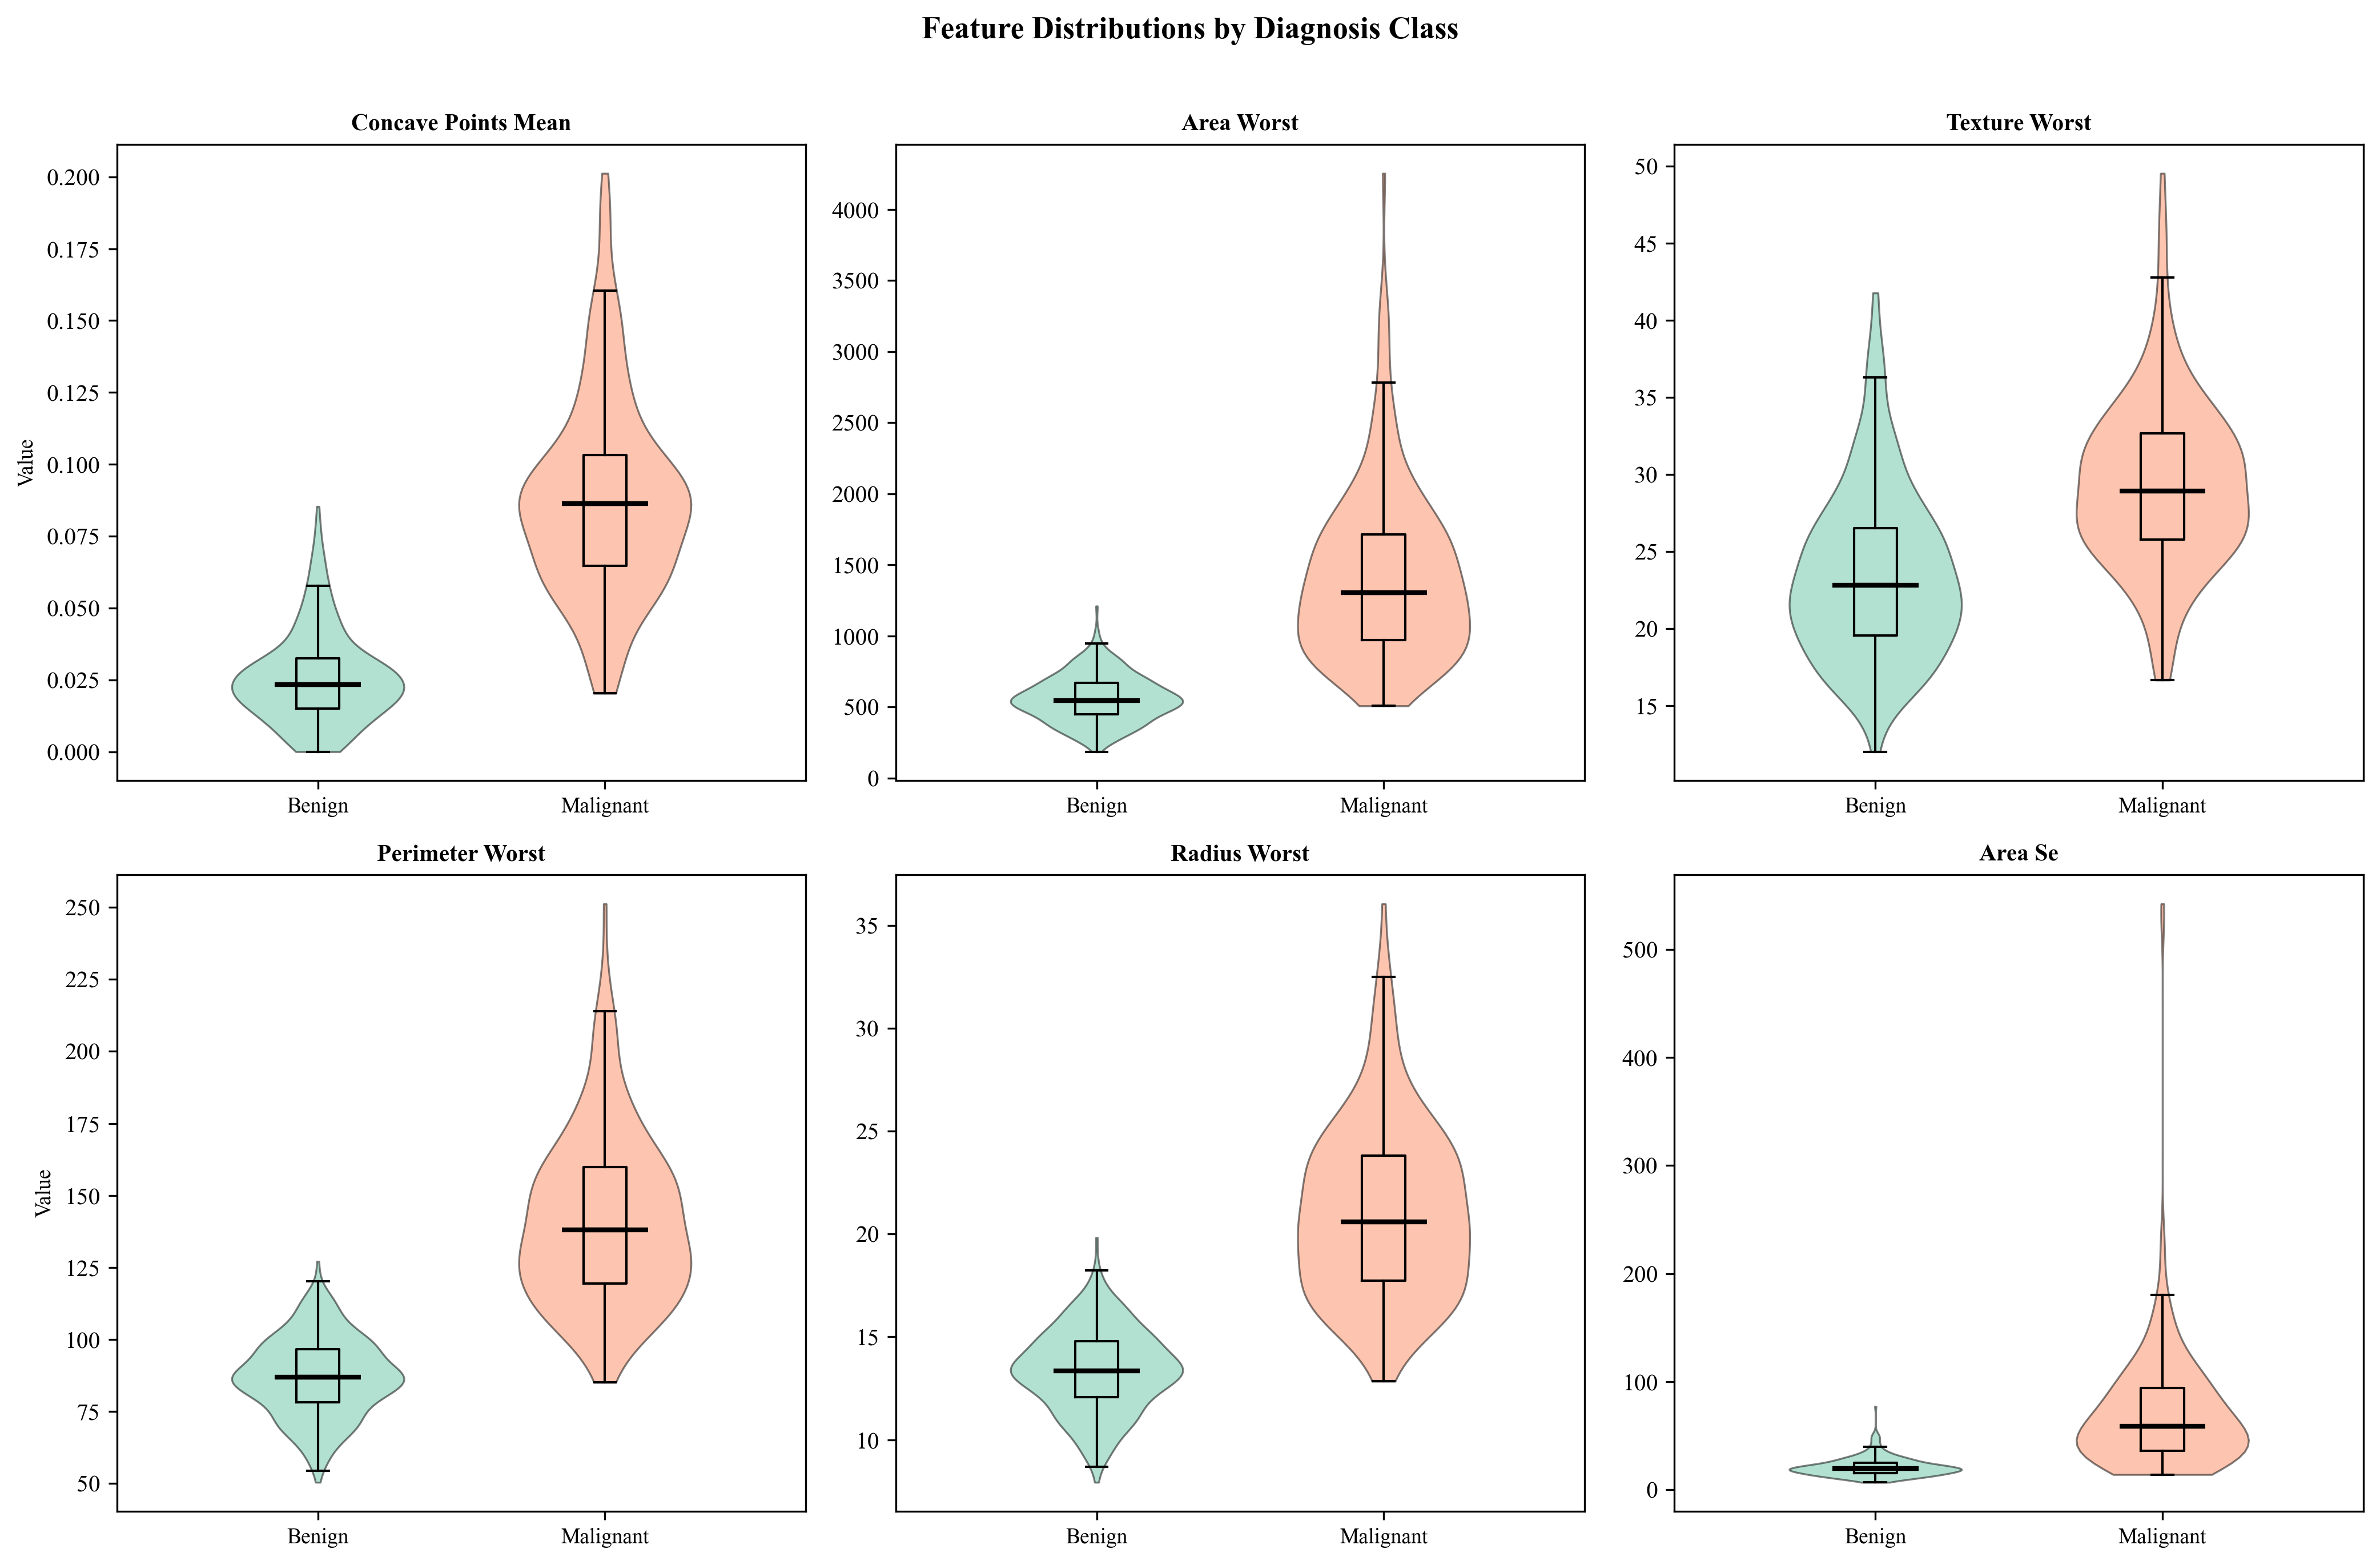
\includegraphics[width=\textwidth]{figures/fig_feature_distributions.png}
\caption{Feature distributions by diagnosis class for the six most discriminative features. Violin plots show the density shape; embedded box plots show median and interquartile range; individual data points are overlaid with low opacity to show sample density.}
\label{fig:distributions}
\end{figure}

The first six principal components capture 90\% of the variance (Kaiser also returns six), and PC1 carries the strongest association with the diagnosis (point-biserial $r=0.78$); ICA, kernel PCA and t-SNE gave the same picture (full redundancy analysis in the repository).

\subsection{Classifier comparison}

Figure~\ref{fig:performance} ranks the top 15 of the 25 model configurations by accuracy on the 143-case test partition; the stacking ensemble, logistic regression L2, SGD, SVM linear and MLP (seed 0) all achieved 141/143 correct.

\begin{figure}[ht!]
\centering
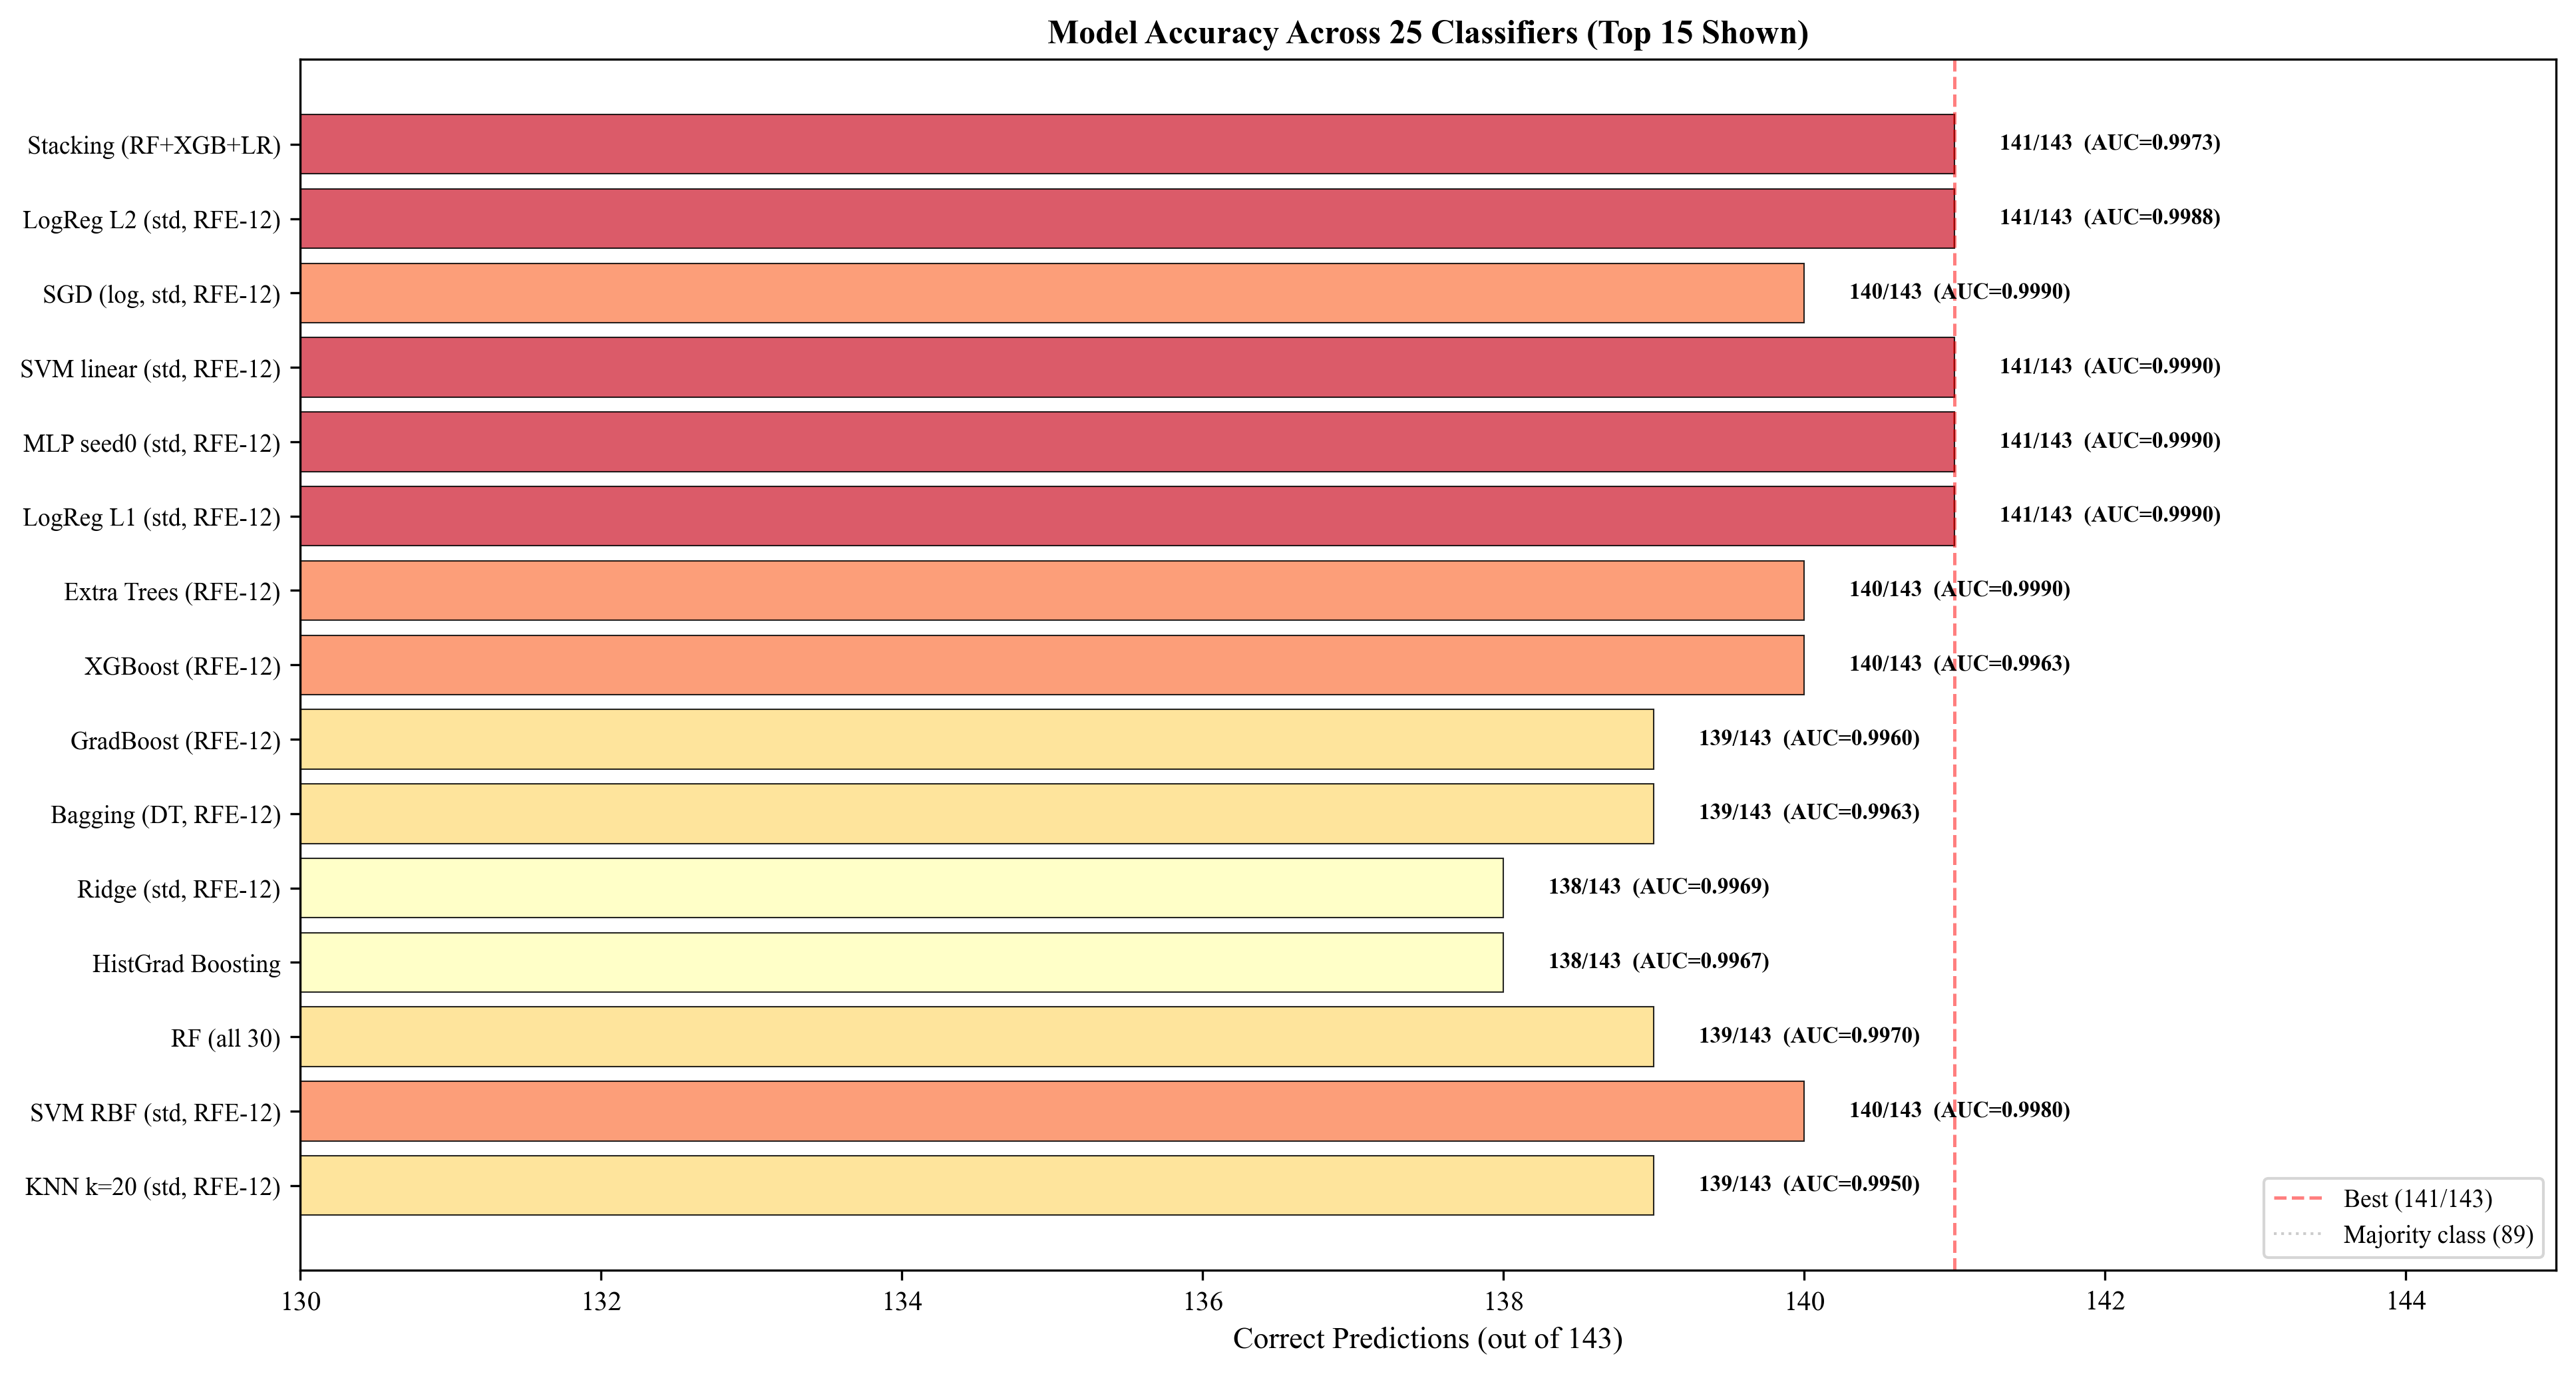
\includegraphics[width=\textwidth]{figures/fig_model_performance.png}
\caption{Model accuracy comparison across the top 15 of 25 model configurations, shown as correct predictions out of 143 test cases. Red bars indicate the best performers (141/143); orange, yellow, and cream indicate progressively lower accuracy. AUC values are shown alongside each bar. The majority-class baseline is 89/143 (62.2\%).}
\label{fig:performance}
\end{figure}

Table~\ref{tab:models} reports the top configurations on the reference partition: stacking and logistic regression L2 (standardised RFE-12) both classified 141 of 143 cases (AUC 0.9973 and 0.9988); SGD achieved the highest AUC (0.9990) with 140/143; the next group scored 138--140.

\begin{table}[ht!]
\centering
\caption{Top-performing configurations on the reference partition (426 training, 143 test). The full 25-model panel is in the accompanying repository \cite{masaba2026code}. Sensitivity is the recall of the malignant class, specificity the recall of the benign class, $FN$ the count of malignant cases called benign. AUC is reported where the model emits a probability or a monotone decision margin; Brier score and expected calibration error for these models appear in the calibration analysis (Figure~\ref{fig:calibration}).}
\label{tab:models}
\renewcommand{\arraystretch}{1.12}
\small
\begin{tabular}{lccccc}
\hline
Model & Correct & Sens. & Spec. & $FN$ & AUC\\
\hline
Stacking (RF+XGB+LR meta) & 141/143 & 0.963 & 1.000 & 2 & 0.9973\\
LogReg L2 (std, RFE-12)   & 141/143 & 0.981 & 0.989 & 1 & 0.9988\\
SGD (log loss, std)       & 140/143 & 0.963 & 0.989 & 2 & 0.9990\\
XGBoost+RFE (native)      & 140/143 & 0.963 & 0.989 & 2 & 0.9963\\
Extra trees (RFE-12)      & 140/143 & 0.963 & 0.989 & 2 & 0.9990\\
HistGradientBoosting      & 138/143 & 0.944 & 0.978 & 3 & 0.9967\\
Bagging (DT base)         & 139/143 & 0.963 & 0.978 & 2 & 0.9963\\
XGBoost (all 30, native)  & 138/143 & 0.944 & 0.978 & 3 & 0.9931\\
\hline
\end{tabular}
\end{table}

The Wilson interval spans 94.0--99.3\% at 141/143, 93.0--98.9\% at 140/143 and 92.1--98.5\% at 138/143, so every interval in the table overlaps every other: the ordering describes one partition, not a ranking of algorithms. The confusion matrices separate the two error types: stacking and logistic regression missed only 1--2 of the 54 malignant cases with 0--1 false alarms, and for triage those are different failures than a single accuracy hides.

Standardisation made a measurable difference for logistic regression: 141/143 standardised vs.\ 138/143 native on RFE-12, a three-case improvement that is not significant on this partition but is consistent with the optimisation landscape (the native-scale fit did not converge within 100 iterations, the standardised version converged in 16).

\subsection{Effect of feature elimination}
\label{sec:elim}

On the reference partition the 12-feature model classified 140 samples against 138 with all 30, two more from 18 fewer measurements, but a margin of two cases is not a result. Over thirty partitions, full averaged 137.2 correct of 143 (sd 2.5) and reduced 137.1 (sd 1.9), a paired difference of $-0.1$ cases (95\% CI $-0.8$ to $+0.5$, treating partitions as independent, which they are not): ahead in 9, behind in 10, level in 11. The reduction is neither a gain nor a loss this dataset can resolve.

That band is narrower than the procedure's own variation: thirty refits with an unseeded wrapper tree returned 137--141 correct and 15 and 19 different twelve-feature subsets across the two batches run in the reference stack. Refitting one model moves the score by four cases; the two models differ by a tenth of a case.

Repeating the experiment on a second numerical stack (xgboost 3.2.0, numpy 2.2.6) moved the paired difference to $-0.9$ cases (interval $-1.5$ to $-0.3$), with 11 distinct subsets across its own refits: the sign is not stable across build environments, which is what a near-zero difference looks like at this size. What the reduction does buy, a decision indistinguishable from the full one from 12 measurements rather than 30, depends on laboratory practice, and no per-assay measurement cost was modelled here.

\begin{table}[ht!]
\centering
\caption{The 12 features retained on the reference partition, grouped by the statistic that summarises each nuclear descriptor. The count in parentheses is the number of the thirty repeated partitions in which the same feature also survived.}
\label{tab:rfe}
\renewcommand{\arraystretch}{1.12}
\begin{tabular}{lll}
\hline
Mean & Standard error & Worst\\
\hline
concave points (14) & area (23) & texture (30)\\
                    & smoothness (11) & perimeter (26)\\
                    & compactness (5) & area (26)\\
                    & concave points (7) & smoothness (20)\\
                    & fractal dimension (16) & radius (20)\\
                    & & compactness (23)\\
\hline
\end{tabular}
\end{table}

Table~\ref{tab:rfe} answers RQ3, but the counts beside each feature answer RQ2 first: one feature was retained in every partition, seven in 20 or more, and two standard-error terms in fewer than ten. The subset is a property of the partition as much as of the data. The correlation structure of Section~\ref{sec:struct} shows many subsets carrying nearly the same information, and a ranking from one decision tree is a weak instrument for choosing among them. Worst-case concave points and concavity were selected in 29 of the 30 partitions, yet neither is in the reference subset.

The instability is not only statistical: changing the numerical library, with the code untouched, replaced two of the twelve features (worst-case concavity and fractal dimension entered; standard-error compactness and fractal dimension left). A subset that is never quite the same twelve features, and scores within two cases each time, is redundancy made visible, so the list should not be read as a finding about which measurements matter clinically. What does hold is the character of the group: six of the twelve are worst-case descriptors, five are standard errors and only one is a mean, concentrating on the tail of the cell population where cytological malignancy is read. A malignant aspirate is identified by its most aberrant nuclei rather than its average, and that worst-case block is also the most stable part of the subset.

\subsection{Explanations and their agreement with the selection}

Ranked by mean absolute contribution over the 143 test cases, the exact SHAP attributions put concave-points mean first by a wide margin (2.20 log-odds), then worst-case texture (1.40), area (1.28) and perimeter (0.83), the remaining eight features contributing under 0.76 each (Figure~\ref{fig:shap}); a single held-out malignant case (predicted probability 0.9995) draws its largest contributions from the same three.

\begin{figure}[ht!]
\centering
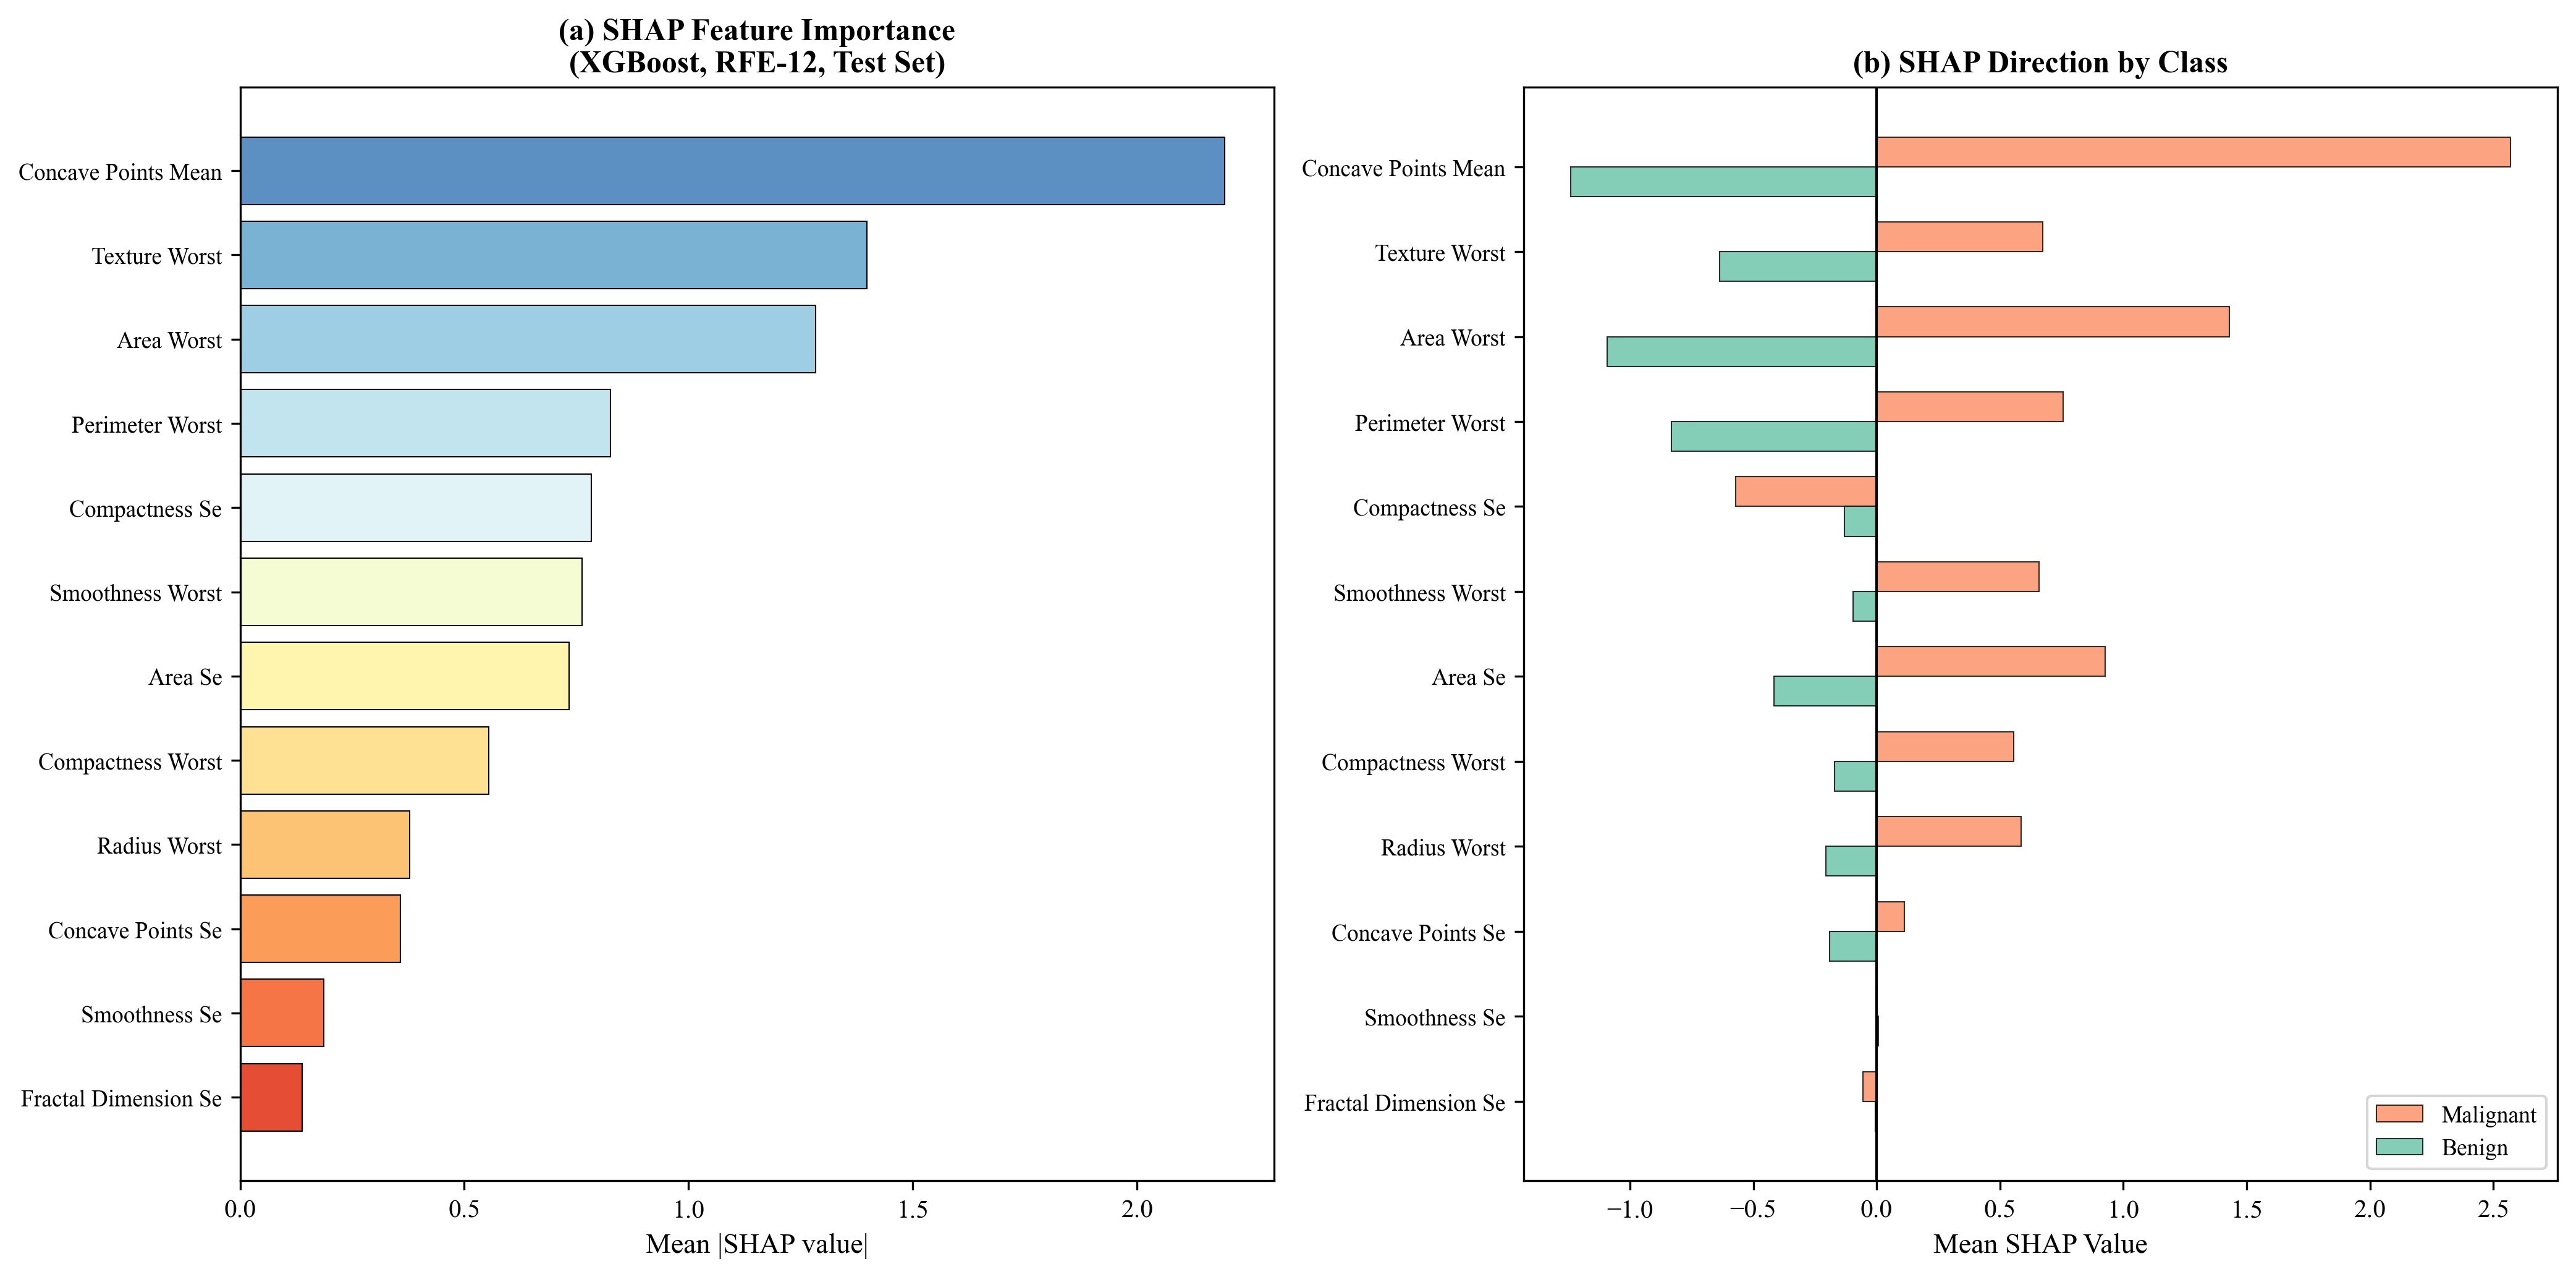
\includegraphics[width=\textwidth]{figures/fig_shap_importance.png}
\caption{SHAP feature importance from exact TreeSHAP on XGBoost (RFE-12, test set). (a) Mean absolute SHAP values for all 12 retained features, ranked by importance. Concave points mean dominates at 2.20, followed by texture worst (1.40) and area worst (1.28). (b) SHAP value direction by class: positive SHAP values push the prediction toward malignant, negative toward benign. The pattern confirms that larger, more irregular nuclei drive malignant predictions.}
\label{fig:shap}
\end{figure}

SHAP interaction values placed 69.6\% of the total $|\phi|$ mass on main effects and 30.4\% on pairs, the strongest being concave points mean $\times$ texture worst (0.44), $\times$ perimeter worst (0.34) and $\times$ radius worst (0.34): concave points mean is modulated by worst-case size and texture. Figure~\ref{fig:logistic} shows the logistic odds ratios; only worst-case texture reaches conventional significance (OR 4.37, 95\% CI [2.32, 8.22], $p=5\times10^{-6}$; Table~\ref{tab:logistic}), but all twelve directions match the cytological account. Several standard-error terms are collinear within the retained set, so their Wald intervals are wide and near-uninformative and only the point estimates and signs should be read.

\begin{figure}[ht!]
\centering
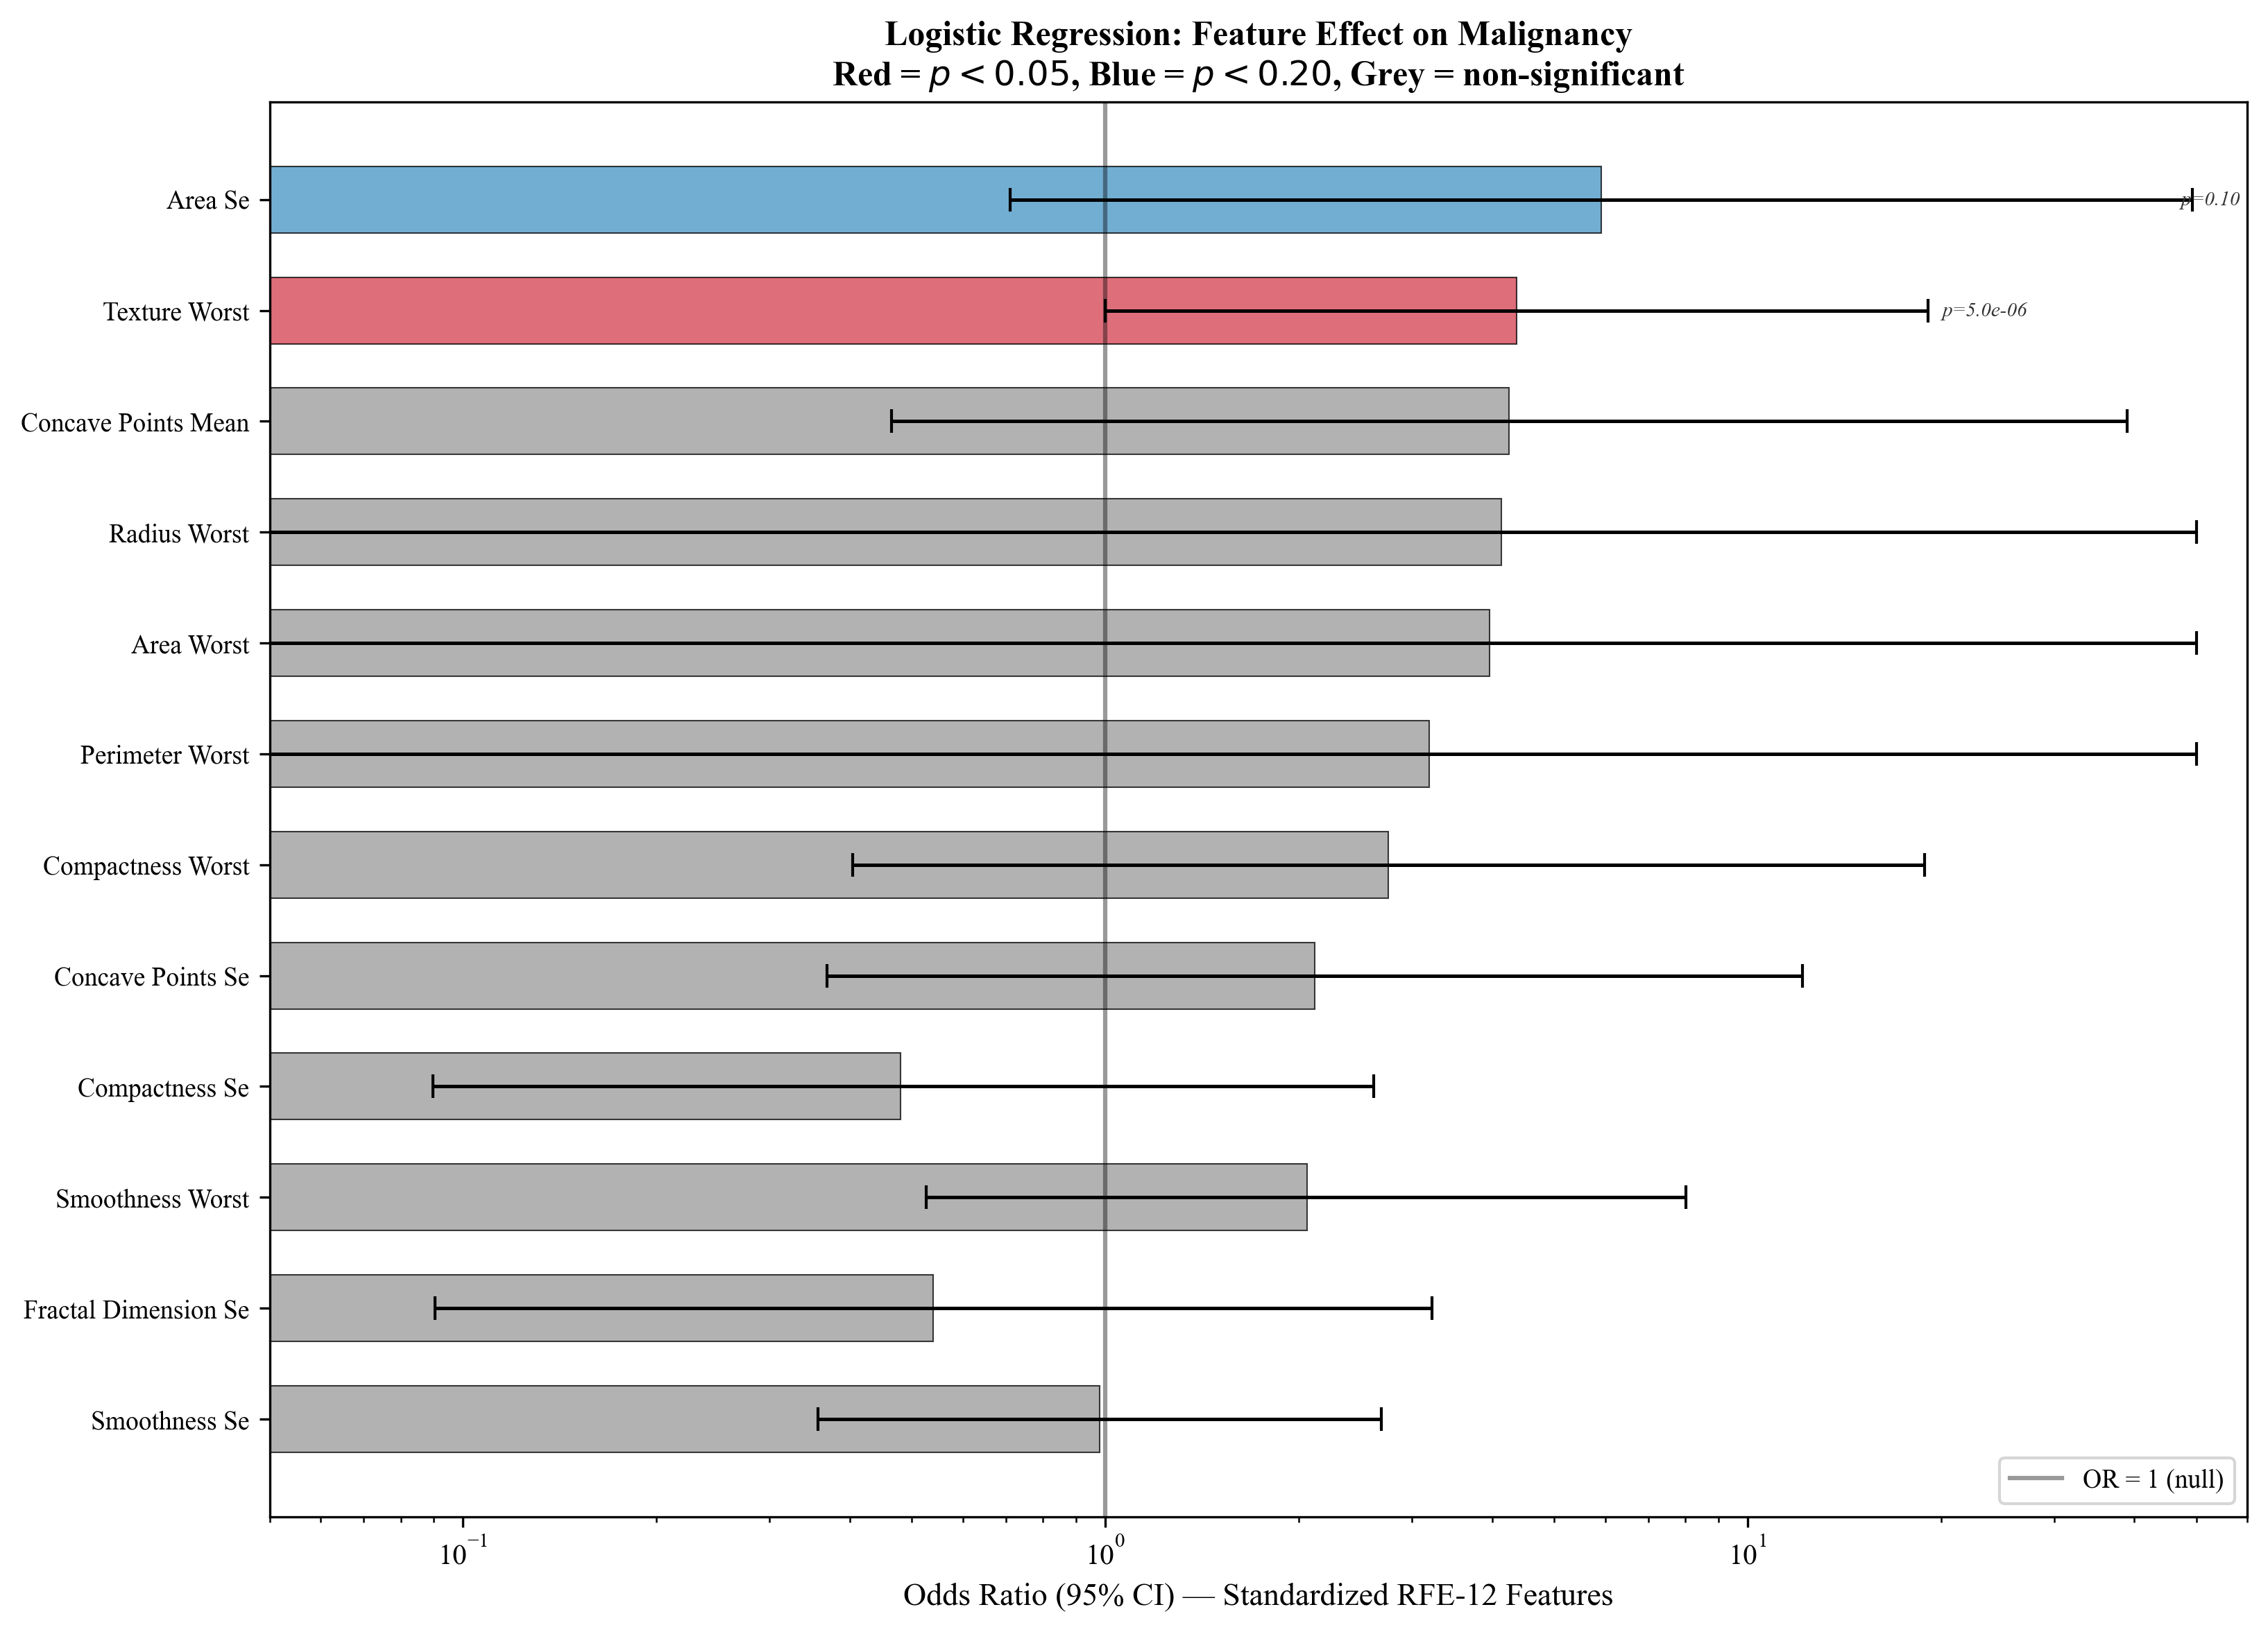
\includegraphics[width=\textwidth]{figures/fig_logistic_coefficients.png}
\caption{Logistic regression odds ratios (95\% Wald CI) for all 12 standardised RFE-12 features. Red bars indicate $p<0.05$; blue indicates $p<0.20$; grey indicates non-significant. Texture worst has the largest significant odds ratio (OR=4.37, $p=5\times10^{-6}$). All positive coefficients indicate features whose increase is associated with malignancy, consistent with the cytological account.}
\label{fig:logistic}
\end{figure}

\begin{table}[ht!]
\centering
\caption{Logistic regression coefficients on standardised RFE-12 features. Beta is the log-odds change per within-cohort standard deviation; OR is exp(beta); CI is the 95\% Wald confidence interval; $p$ is the two-sided Wald test.}
\label{tab:logistic}
\renewcommand{\arraystretch}{1.12}
\small
\begin{tabular}{lcccc}
\hline
Feature & Beta & OR & CI & $p$\\
\hline
area\_se            & +1.778 & 5.92 & [0.57, 60.97] & 0.1\\
texture\_worst      & +1.475 & 4.37 & [2.32, 8.22]  & 5e-06\\
concave points\_mean & +1.448 & 4.25 & [0.51, 35.20] & 0.2\\
radius\_worst       & +1.421 & 4.14 & [0.00, 4180731] & 0.8\\
area\_worst         & +1.379 & 3.97 & [0.00, 11693073] & 0.9\\
perimeter\_worst    & +1.159 & 3.19 & [0.00, 11148] & 0.8\\
compactness\_worst  & +1.016 & 2.76 & [0.38, 20.23] & 0.3\\
concave points\_se  & +0.751 & 2.12 & [0.35, 12.91] & 0.4\\
compactness\_se     & $-0.724$ & 0.48 & [0.08, 3.05] & 0.4\\
smoothness\_worst   & +0.720 & 2.06 & [0.54, 7.75] & 0.3\\
fractal dimension\_se & $-0.615$ & 0.54 & [0.09, 3.23] & 0.5\\
smoothness\_se      & $-0.019$ & 0.98 & [0.29, 3.34] & 1.0\\
\hline
\end{tabular}
\end{table}

Exact permutation importance (50 shuffles per column, seed 0) places the largest cross-family accuracy drops on concave points mean (0.036) and texture worst (0.028), then perimeter worst (0.018) and area worst (0.017). XGBoost loses 0.083 accuracy when concave points mean is shuffled; random forest and extra trees redistribute the signal across correlated columns and produce flatter bars, with maximum drops of 0.015 and 0.020 respectively. Rank agreement with the SHAP ordering is $\rho=+0.92$ for XGBoost, $+0.73$ for extra trees, $+0.70$ for random forest, $+0.59$ for the standardised logistic model. Two features, smoothness standard error and fractal dimension standard error, have zero mean drop in every family (Figure~\ref{fig:perm}).

\begin{figure}[ht!]
\centering
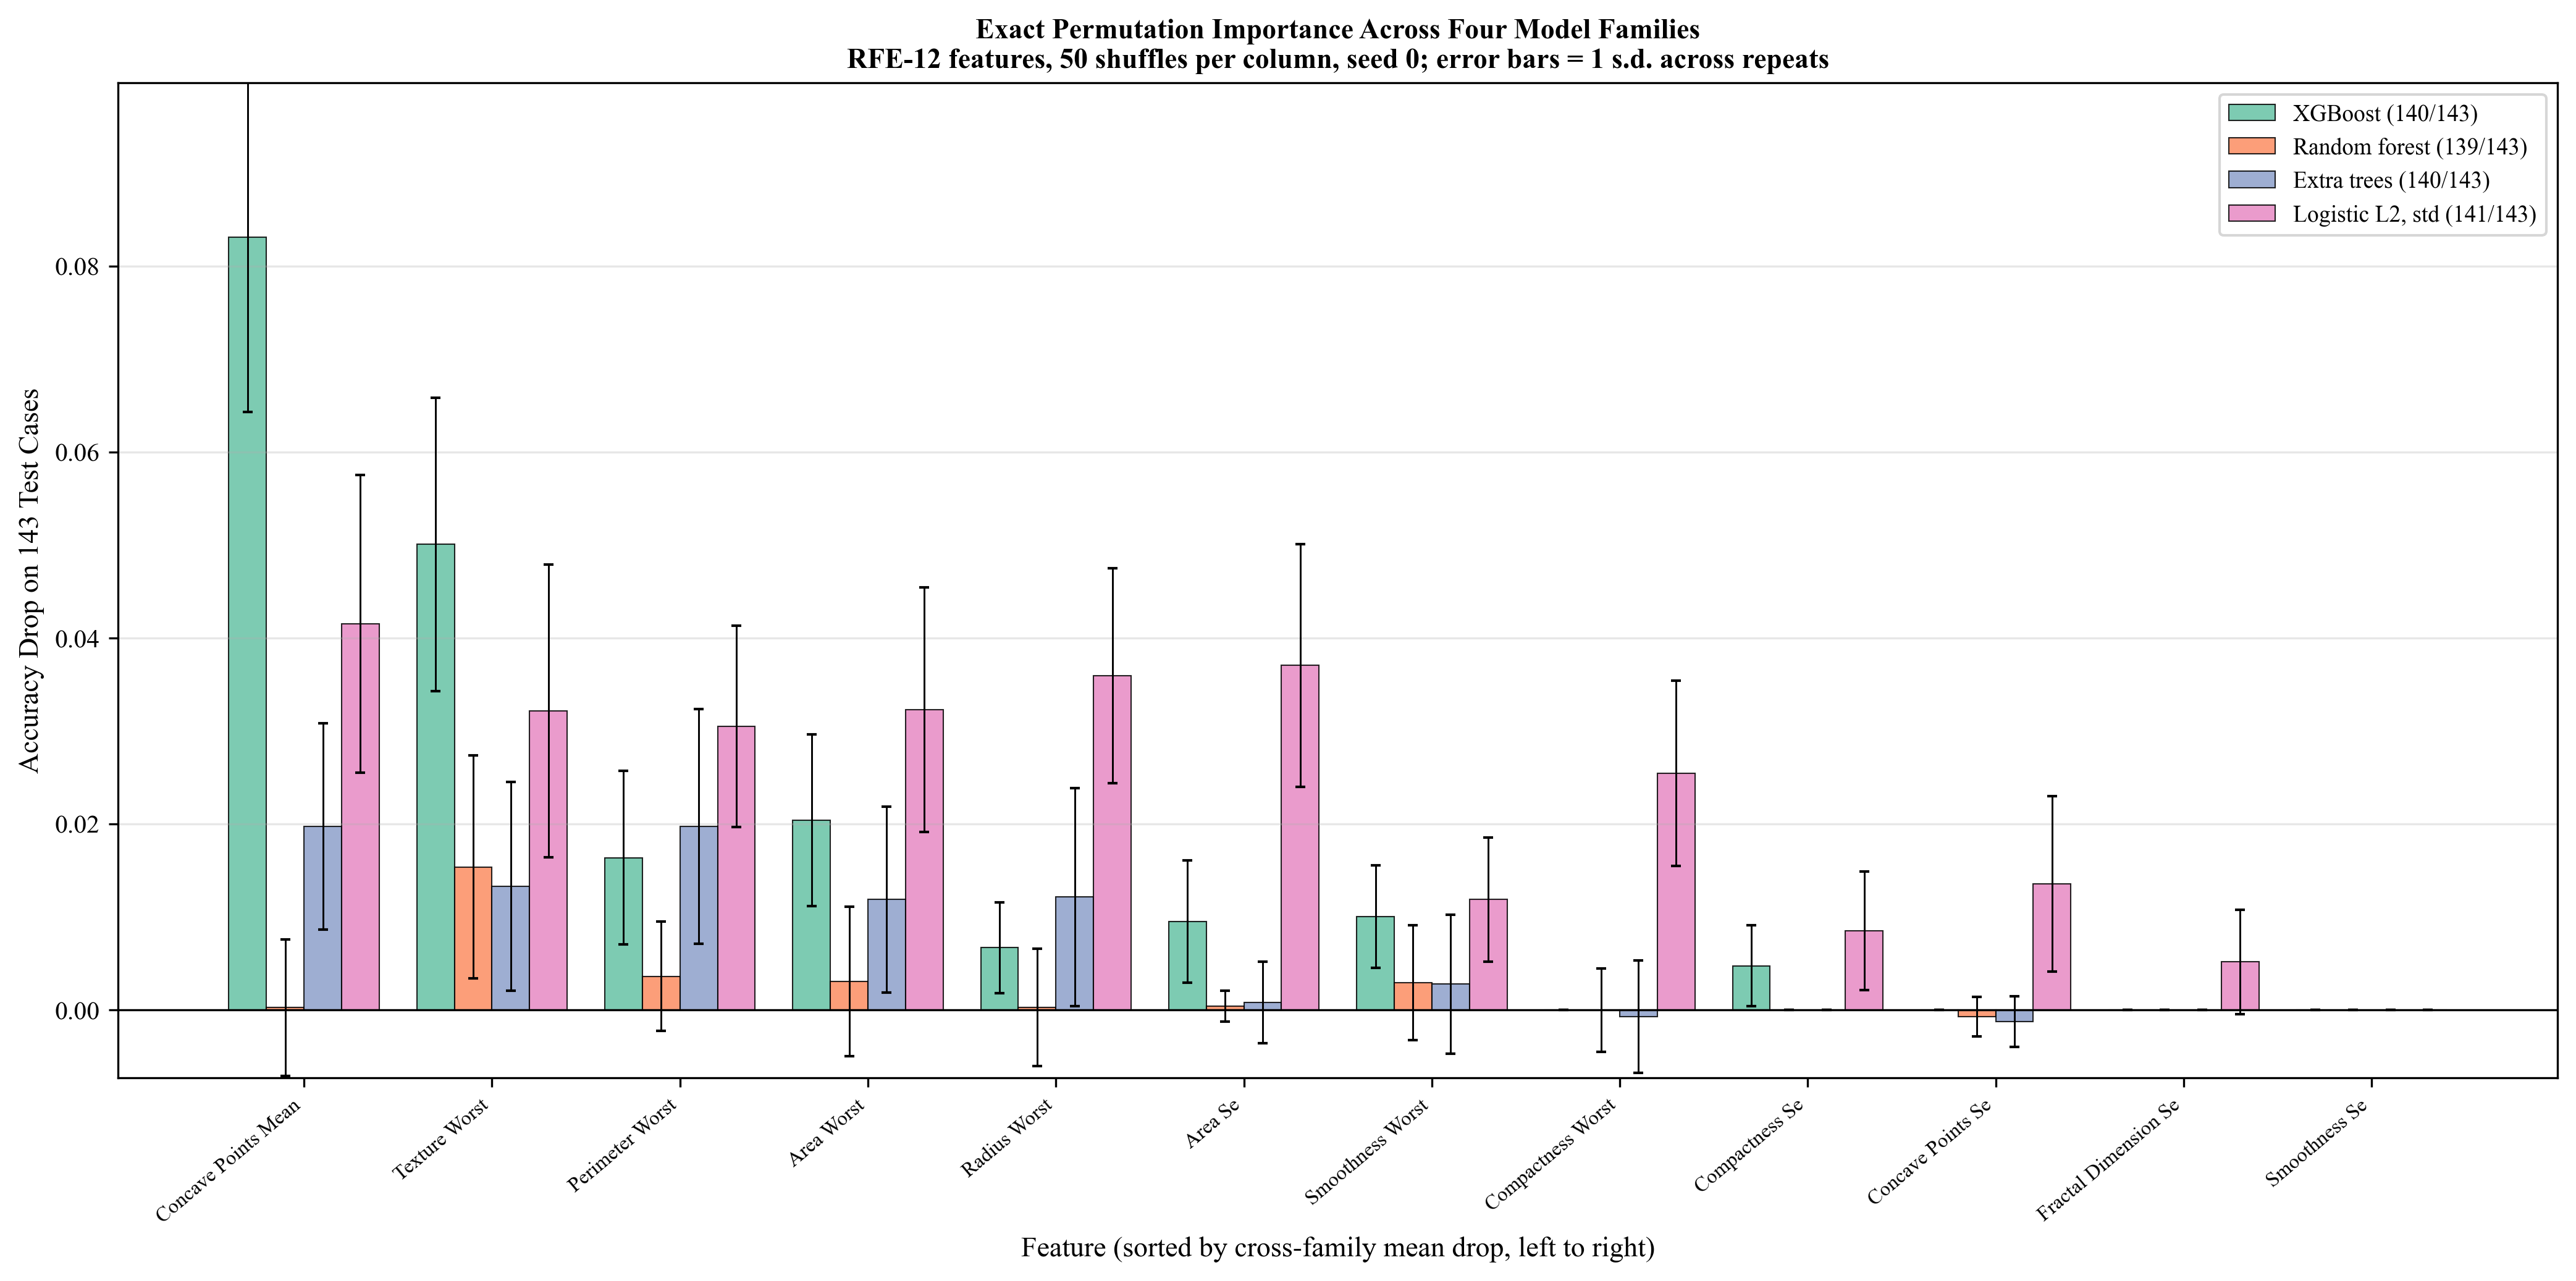
\includegraphics[width=\textwidth]{figures/fig_permutation_importance.png}
\caption{Exact permutation importance across four model families on the RFE-12 features (50 shuffles per column, seed 0; bars show the mean accuracy drop on the 143 test cases, error bars one standard deviation across repeats). Concave points mean dominates every family that reads it; random forest and extra trees show flatter bars because their ensembles redistribute the signal across correlated columns. Smoothness standard error and fractal dimension standard error contribute nothing under any family.}
\label{fig:perm}
\end{figure}

Figure~\ref{fig:consensus} compares the four global-importance views used here (exact SHAP, permutation importance, logistic $|\beta|$ and a univariate AUC screen); partial dependence and LIME describe response shape and per-case locality rather than a single global ranking, so they are reported separately above and in the repository.

\begin{figure}[ht!]
\centering
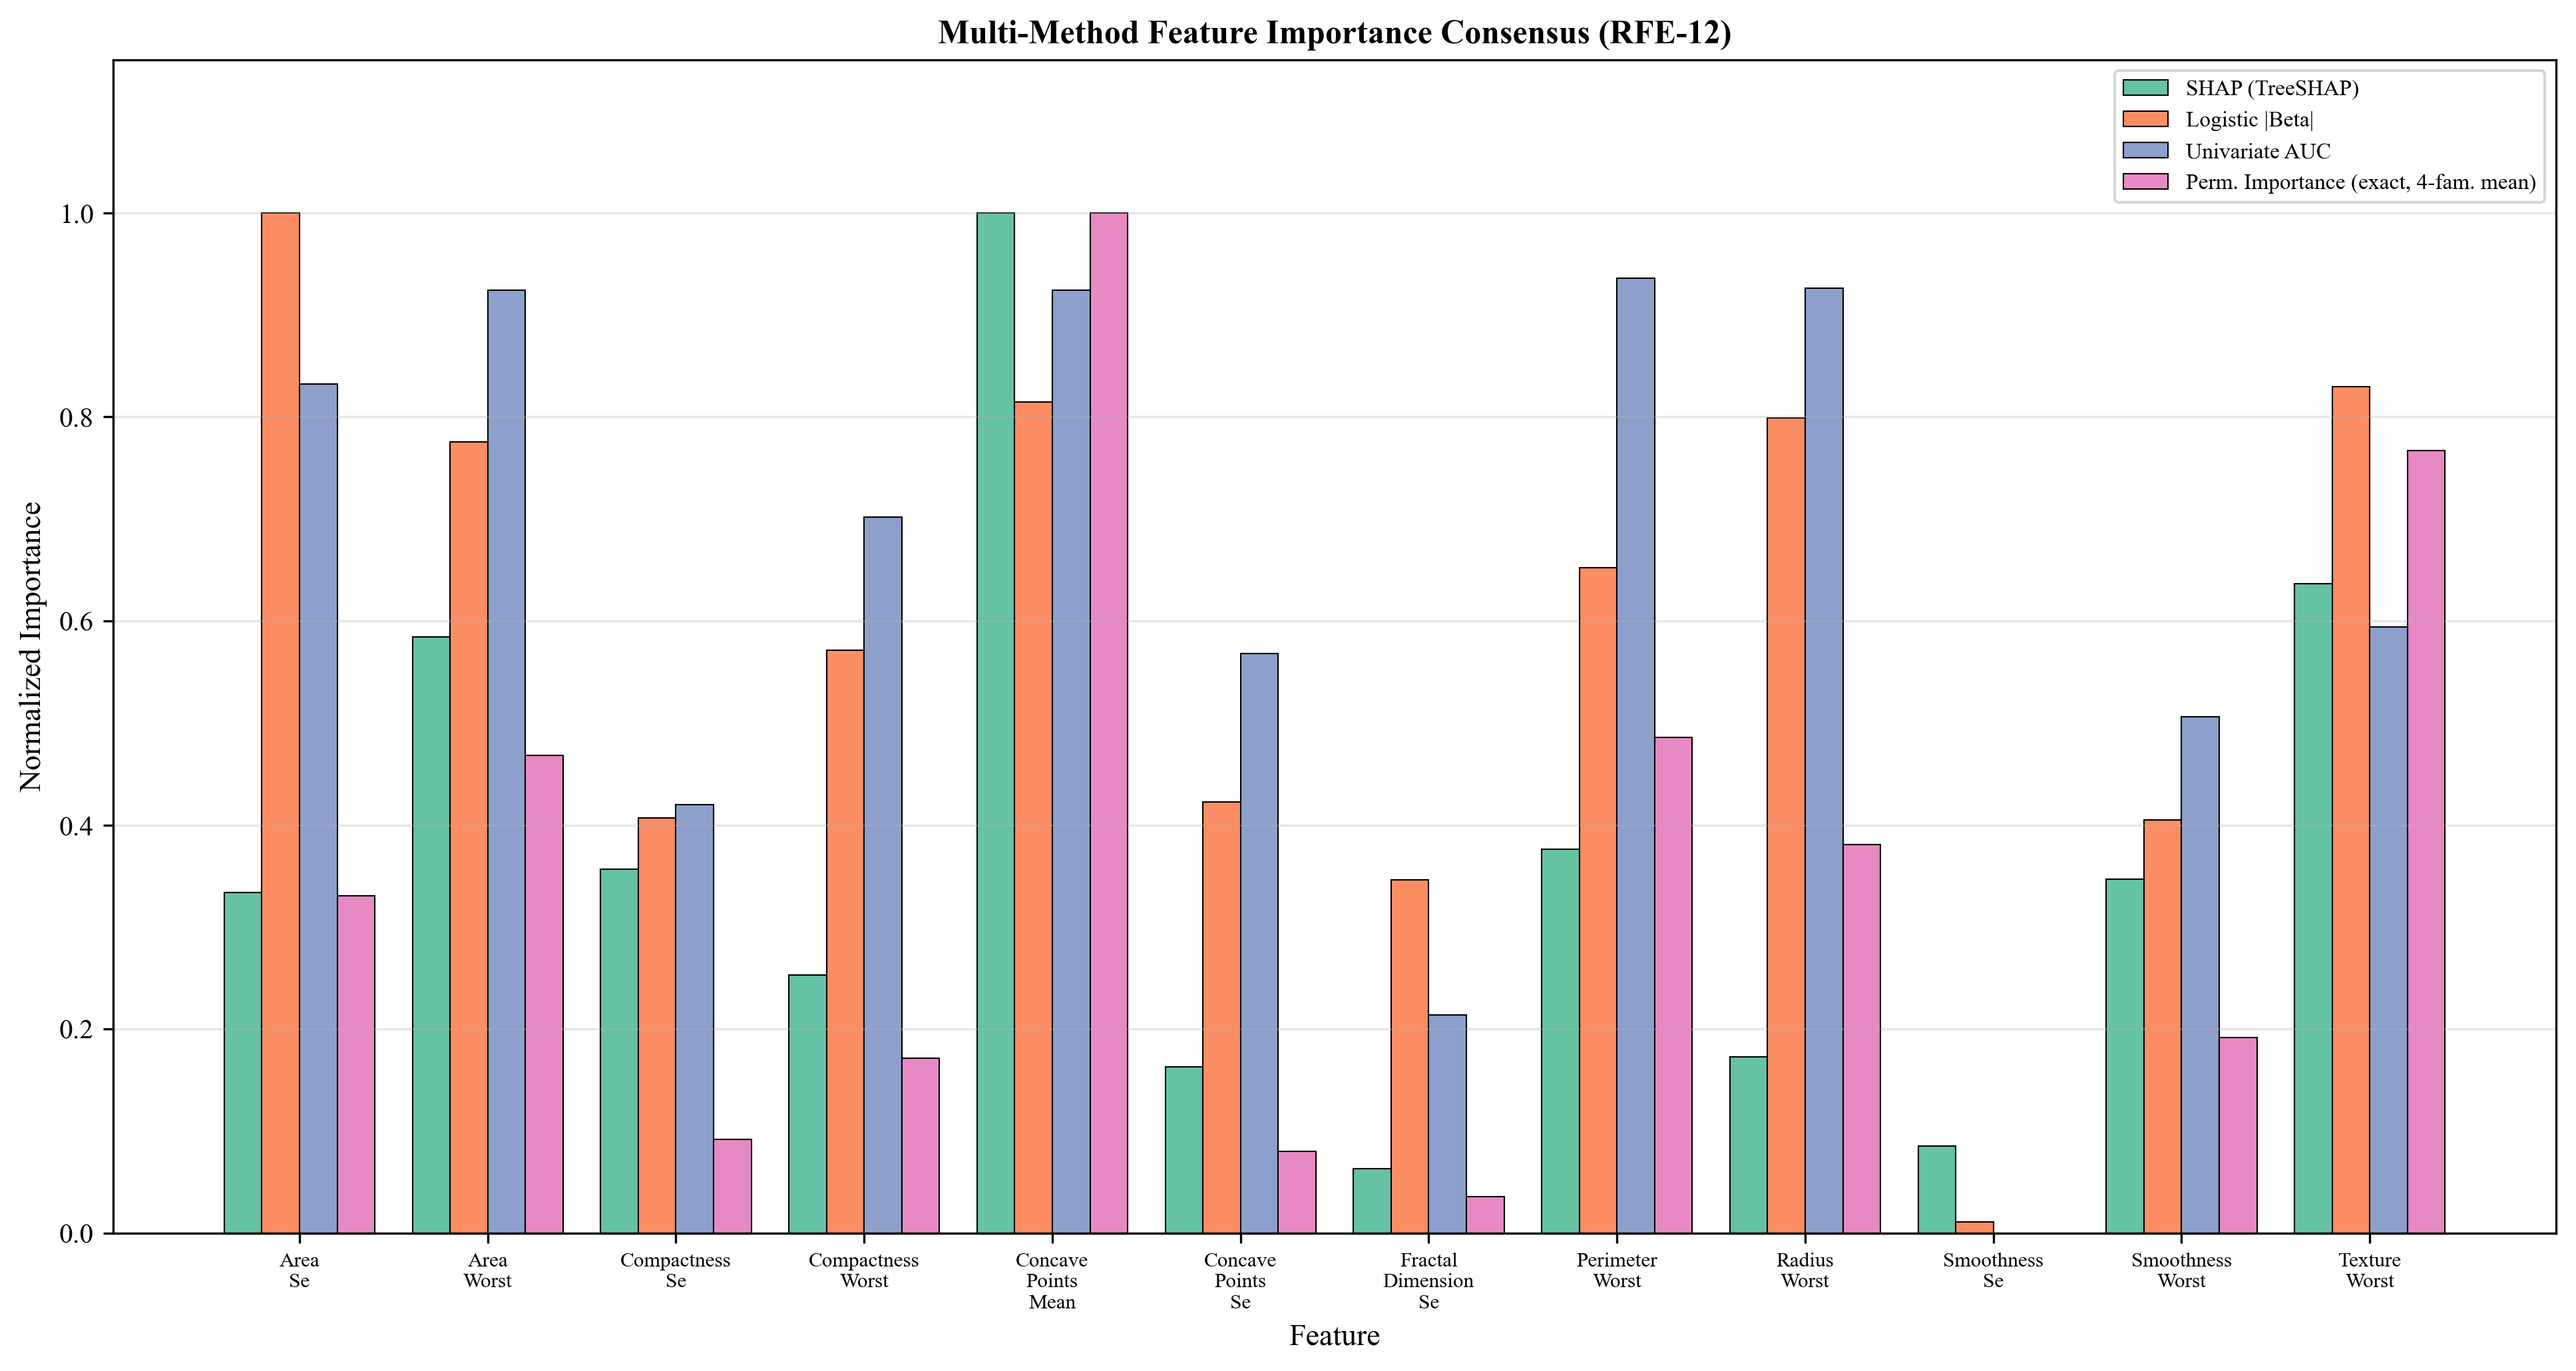
\includegraphics[width=\textwidth]{figures/fig_importance_consensus.png}
\caption{Multi-method feature importance consensus plot showing normalised importance scores from SHAP (TreeSHAP), logistic regression coefficients ($|\beta|$), univariate AUC, and the exact permutation importance of Fig.~\ref{fig:perm} (mean across the four families, rescaled to its maximum). All four methods place concave points mean and texture worst among the leading predictors, with area worst and perimeter worst close behind, providing converging evidence for the retained feature set.}
\label{fig:consensus}
\end{figure}

Partial dependence plots confirmed monotone increases in predicted malignancy for the top four features, and LIME stability gave top-5 Jaccard indices of 0.60--0.80, naming the same leading features across seeds. RQ4 is thus answered affirmatively, with a qualification: all five methods read the same fitted model, so their agreement is weaker evidence than it appears (consistency does not make a feature causal), but the internal coherence matches the cytological account of a malignant aspirate.

\subsection{Protocol validation results}

Figure~\ref{fig:cv} shows the results. Logistic regression with all 30 standardised features achieved the highest mean fold accuracy (0.976, a mean of 111.0 correct of the $\approx$113.8 held-out cases per fold), followed by MLP with all 30 standardised (0.976), logistic regression with RFE-12 standardised (0.973) and SVM linear with all 30 standardised (0.973); XGBoost scored 0.967 (all 30, native) and 0.964 (RFE-12, native).

The paired comparison across folds showed that the reduction from 30 to 12 features (XGBoost, native) was not significant ($-0.05$ percentage points, 95\% CI $[-0.17, +0.07]$, paired $t$-test $p=0.400$), confirming the single-partition finding that the reduction costs nothing, while standardisation significantly improved logistic regression (standardised RFE-12 minus native all-30: $+0.41$ percentage points, 95\% CI $[+0.27, +0.55]$, paired $t$-test $p<0.001$).

\begin{figure}[ht!]
\centering
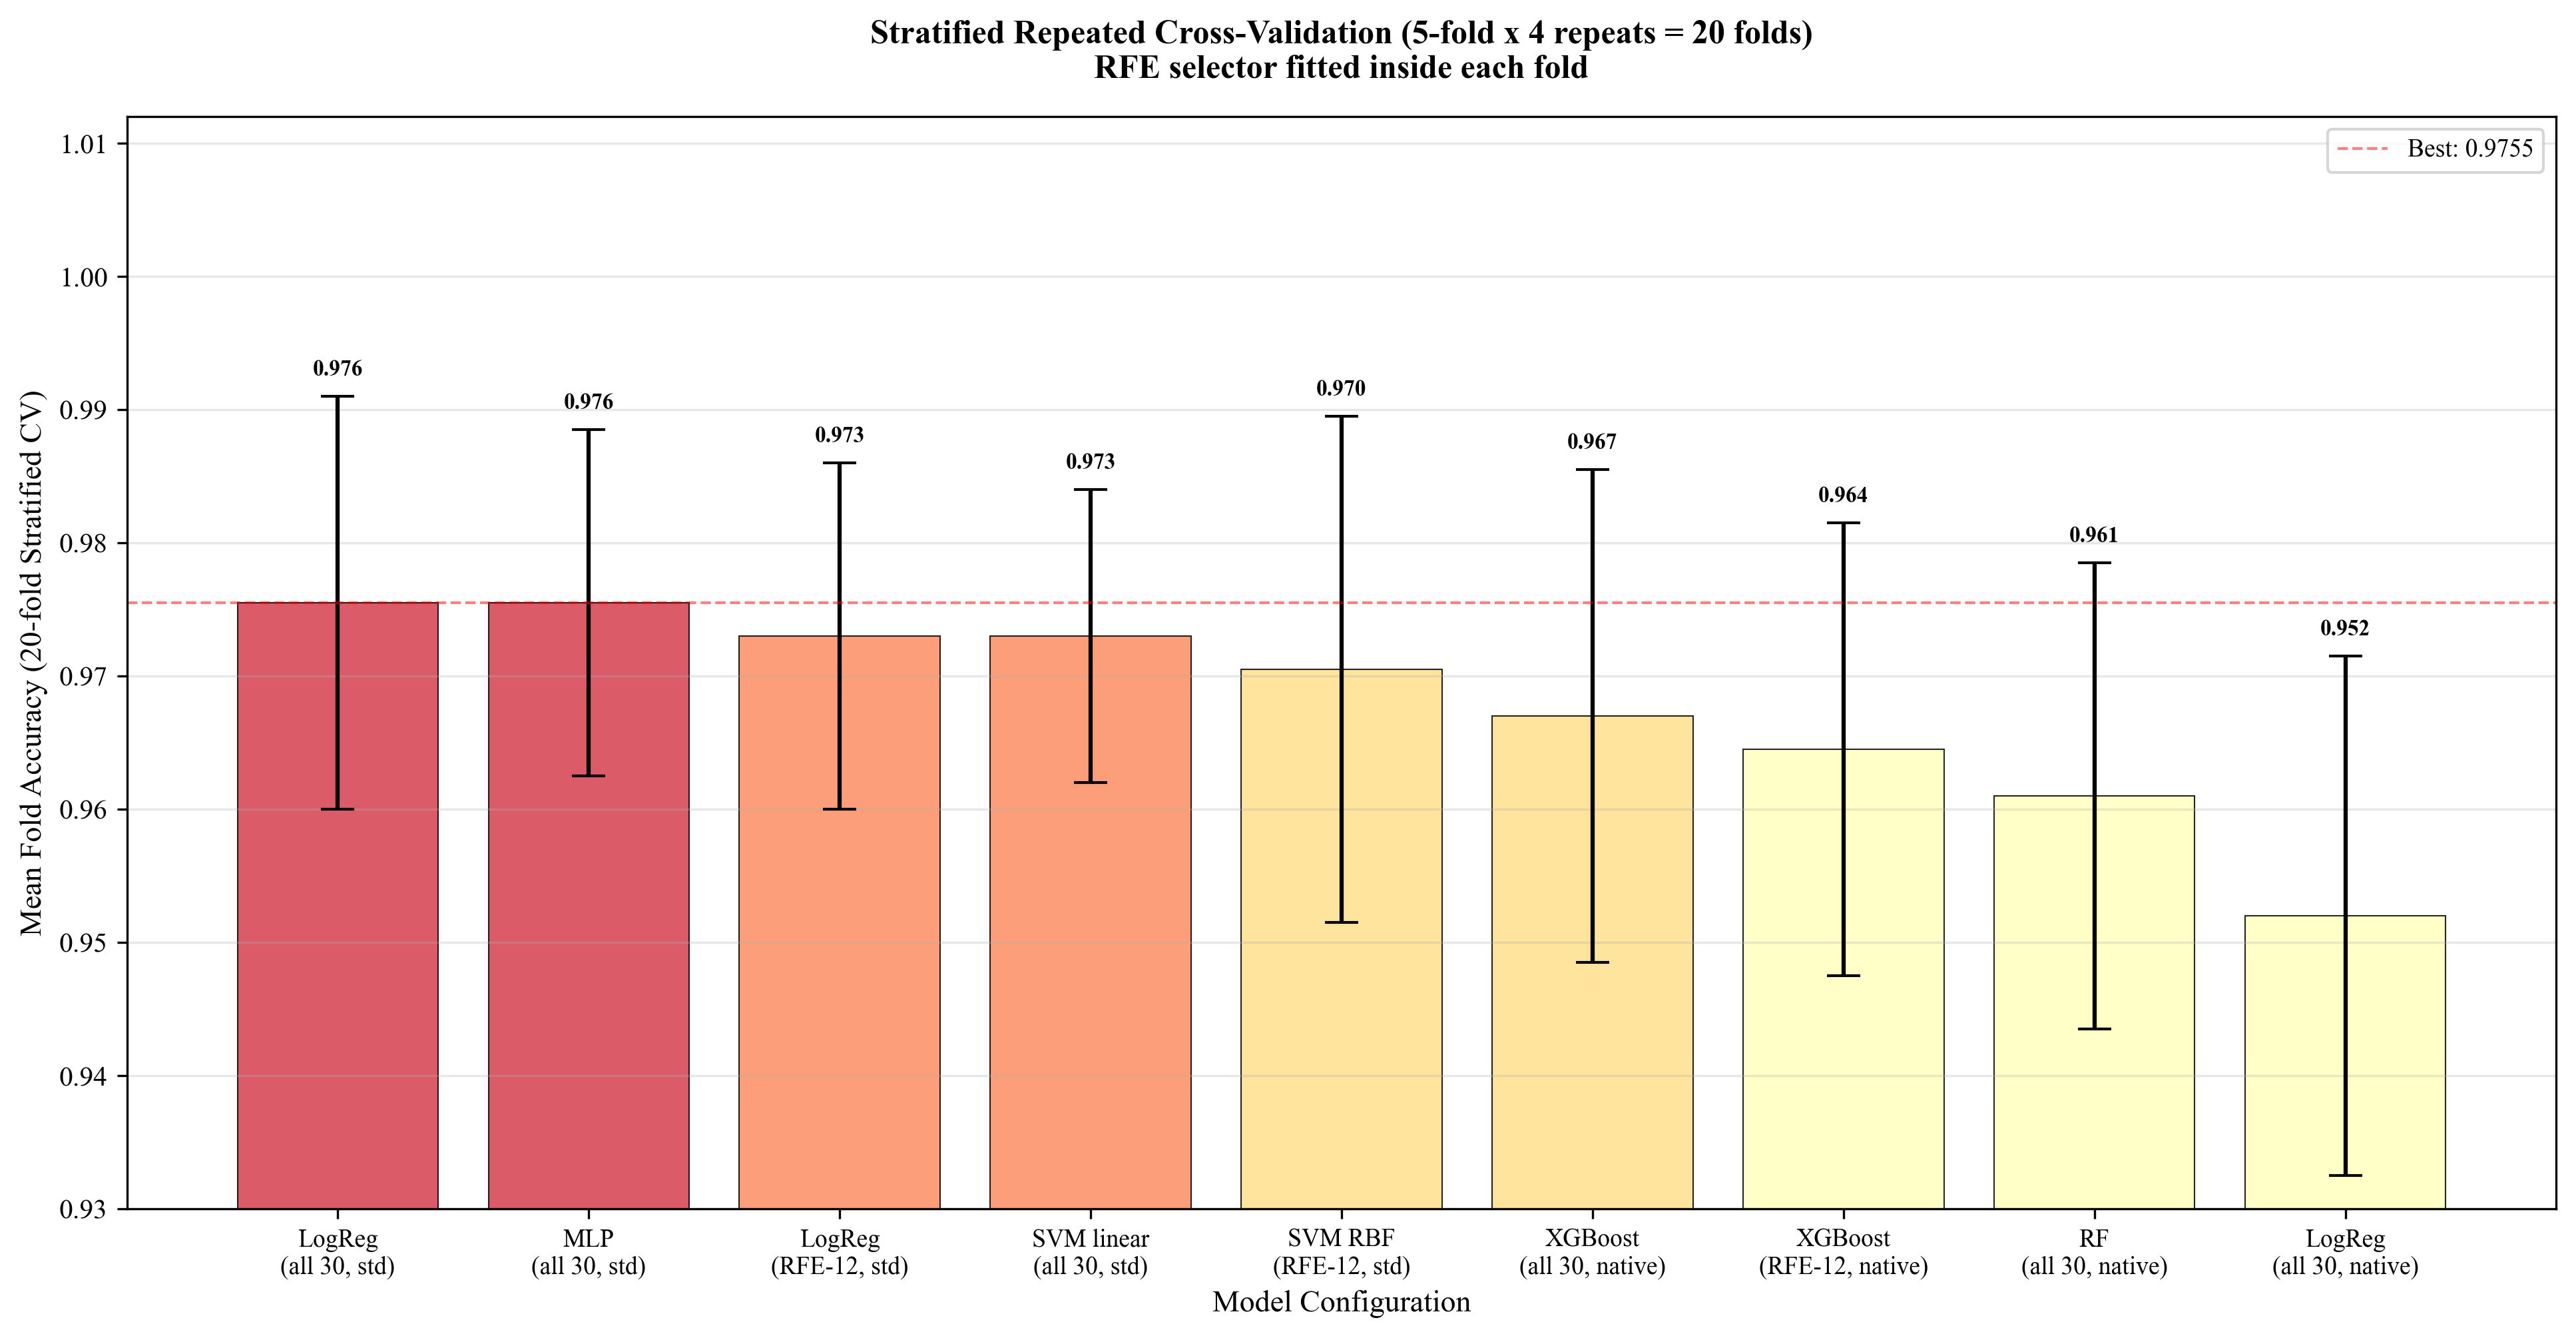
\includegraphics[width=\textwidth]{figures/fig_stratified_cv.png}
\caption{Stratified repeated cross-validation results (5-fold $\times$ 4 repeats = 20 folds) with the RFE selector fitted inside each fold. Bars show mean held-out fold accuracy; error bars show $\pm 1$ standard deviation across folds. Logistic regression (all 30, standardised) and MLP (all 30, standardised) achieve the highest mean fold accuracy (0.976, a mean of 111.0 correct out of the $\approx$113.8 held-out cases per fold). The RFE selector is fitted blind to each held-out fold.}
\label{fig:cv}
\end{figure}

The RFE-$k$ sweep (20 stratified folds per $k$; Figure~\ref{fig:rfe}) showed that $k=12$ is near-optimal: logistic regression (standardised) scored a mean of 111.0 correct per fold at $k=12$ and 111.2 at $k=16$ (not significantly better) against 110.2 at $k=4$, and the overlap of the selected set with the reference twelve grew monotonically from 4 of 12 at $k=4$ to 12 of 12 at $k=12$, confirming that the selector stabilises at this size.

\begin{figure}[ht!]
\centering
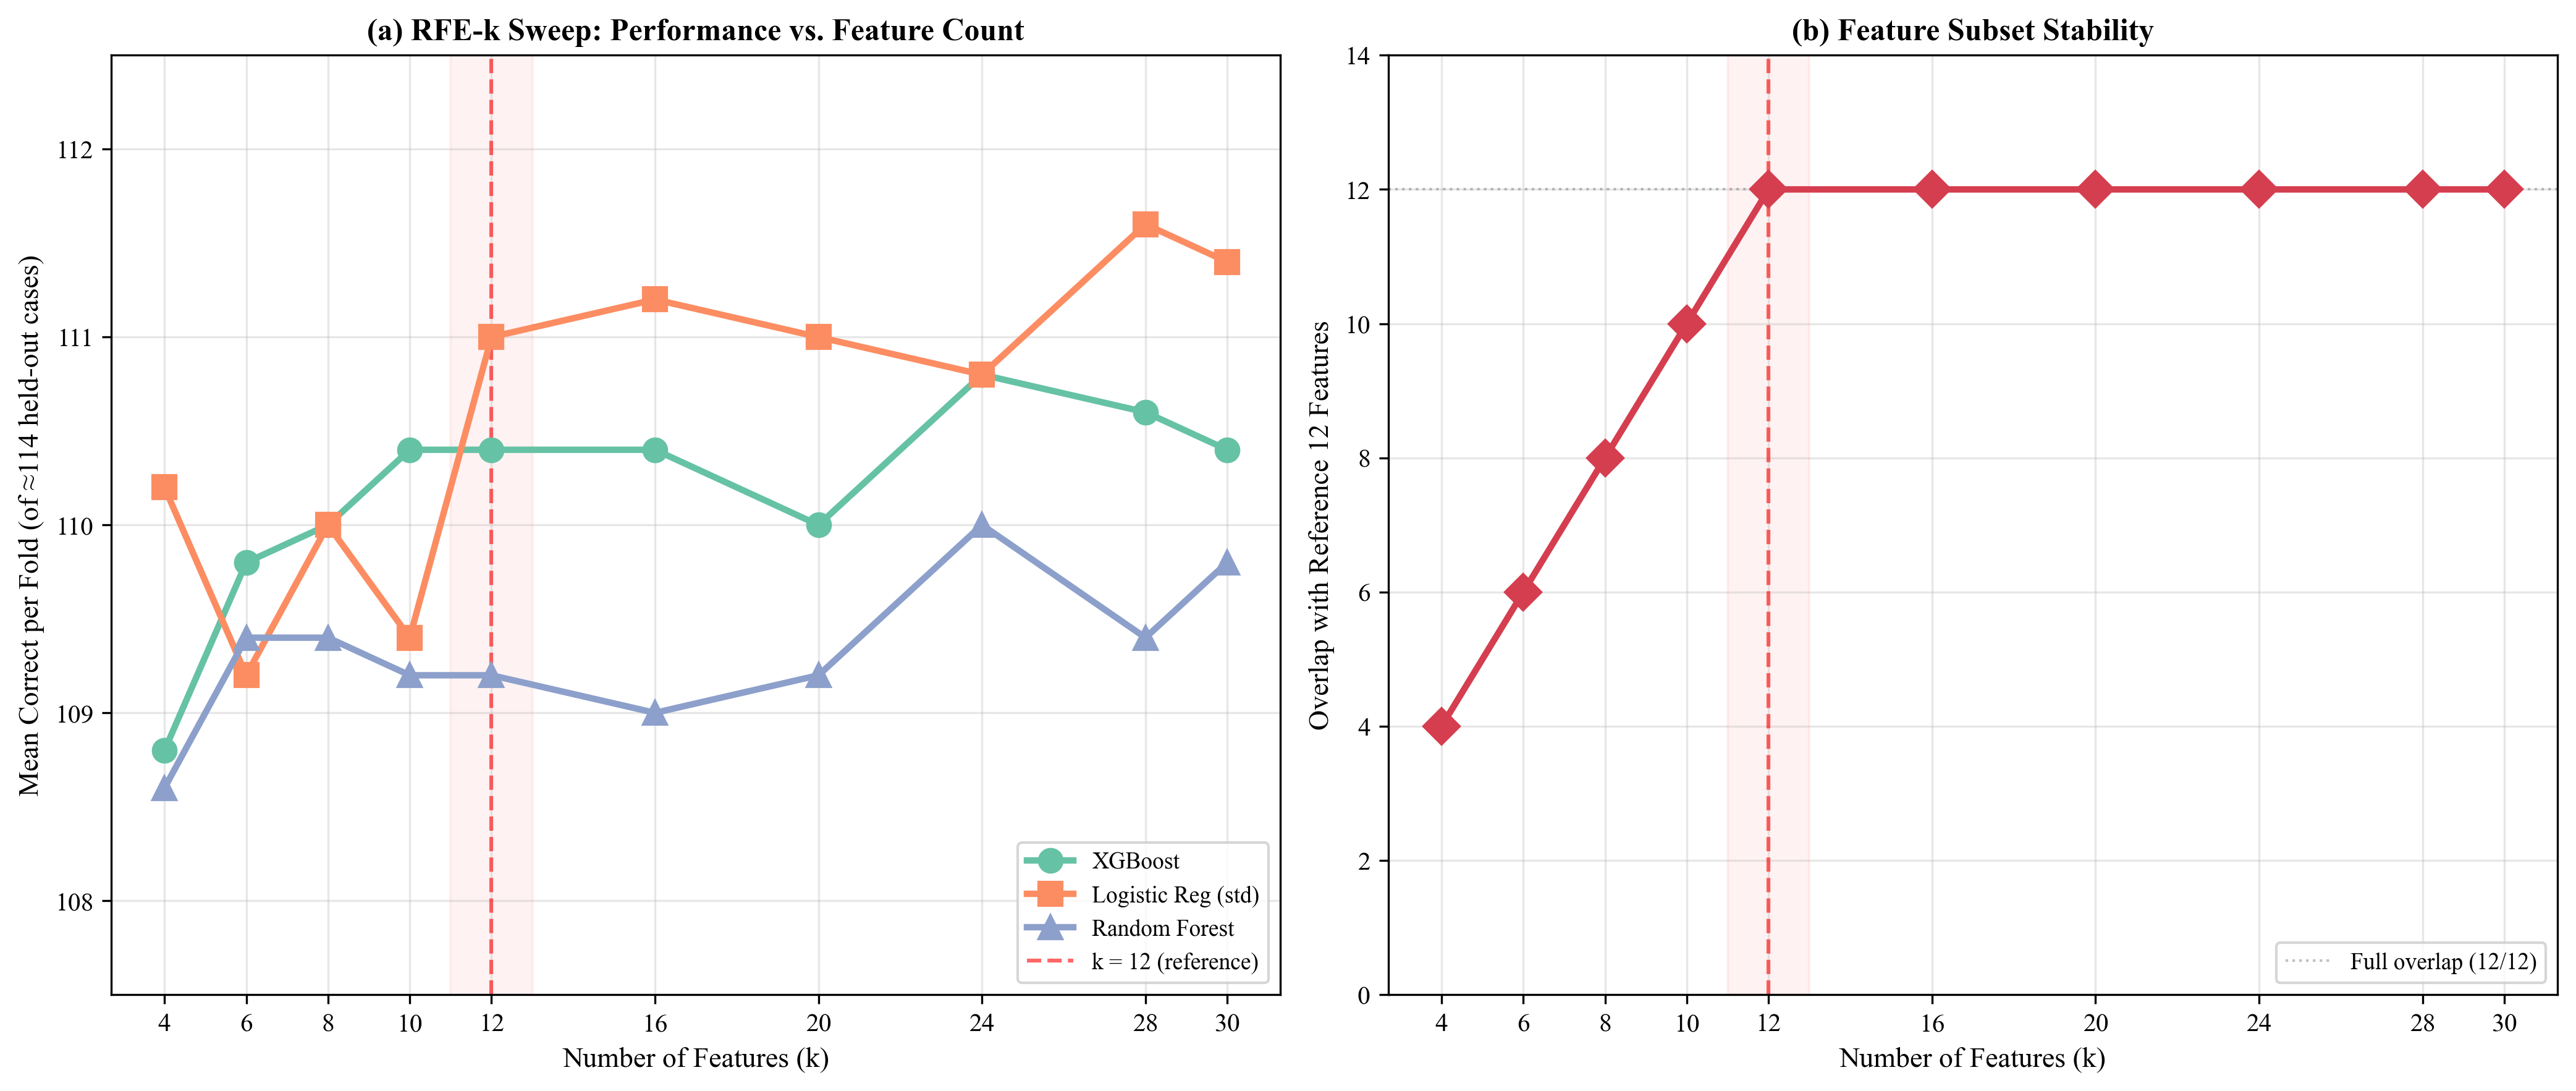
\includegraphics[width=\textwidth]{figures/fig_rfe_k_sweep.png}
\caption{RFE-$k$ sweep: (a) classification performance (mean correct predictions per fold, out of $\approx$114 held-out cases, 20-fold CV) as a function of the number of retained features $k$, for XGBoost, logistic regression (standardised), and random forest. The red dashed line marks $k=12$ (the reference). Performance is near-optimal at $k=12$ for all three families. (b) Feature subset stability: overlap of the selected $k$-feature set with the reference 12-feature set. The overlap reaches 12/12 at $k=12$ and stays there, confirming that the selector stabilises at this size.}
\label{fig:rfe}
\end{figure}

Nested tuning identified the optimal configurations: SVM with scaling chose $C=0.1$, linear kernel in 3 of 5 folds (111.0 correct per fold); logistic regression chose $C=0.1$, L2 in 4 of 5 folds (111.4, the best); MLP chose a hidden layer of 100 units in all folds (107.2). Defaults are near-optimal for logistic regression and MLP here.

\subsection{Model agreement and consensus analysis}

\begin{figure}[ht!]
\centering
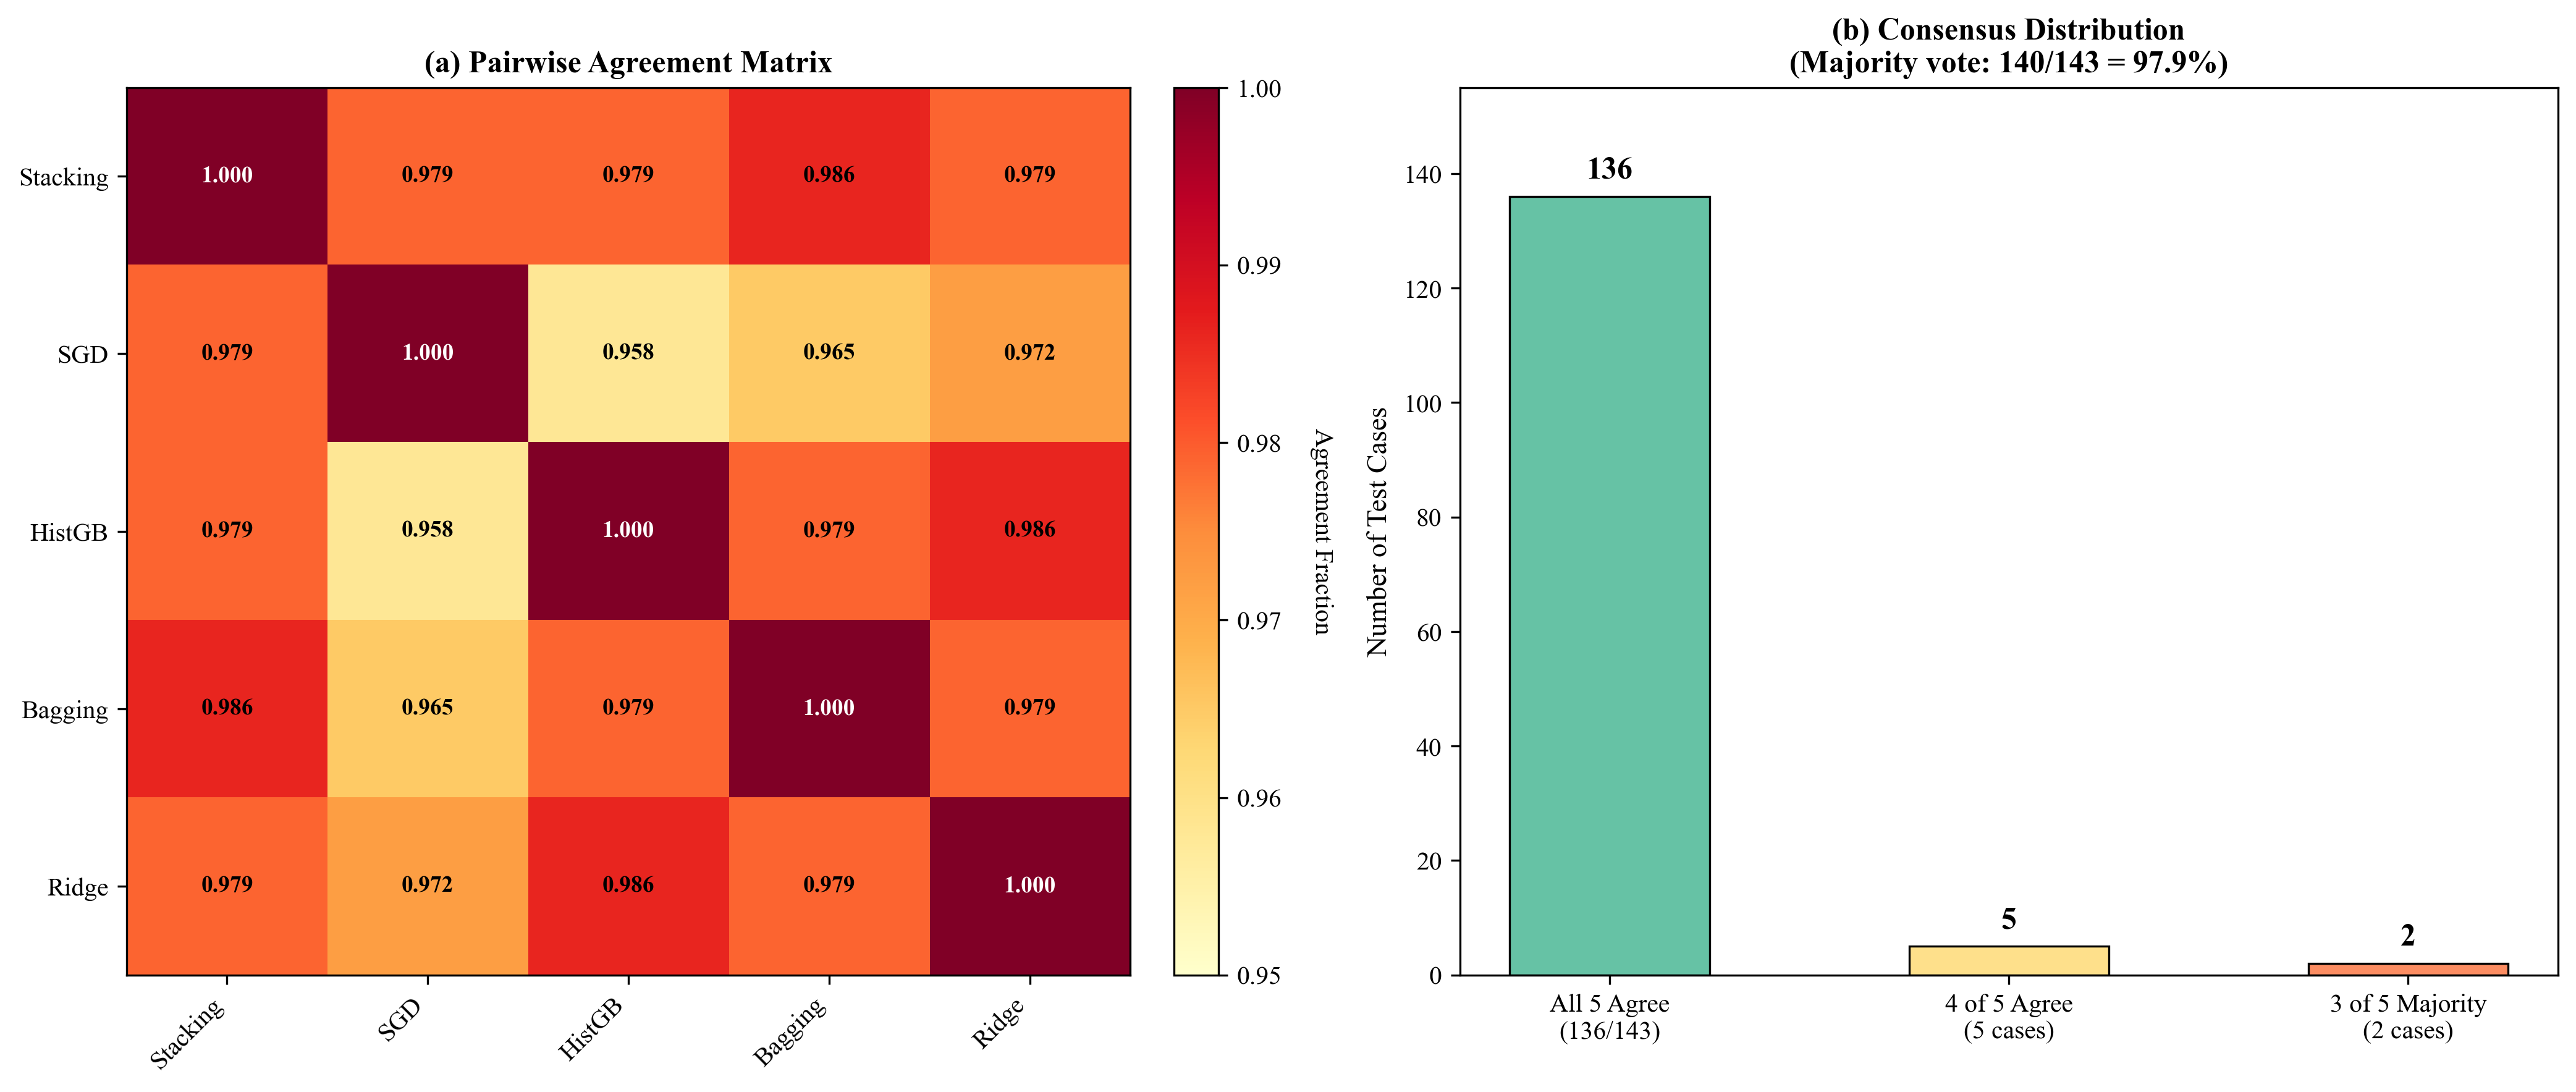
\includegraphics[width=\textwidth]{figures/fig_model_agreement.png}
\caption{Model agreement analysis across five ensemble variants (stacking, SGD, histogram-based gradient boosting, bagging, ridge classifier). (a) Pairwise agreement matrix: fraction of 143 test cases where each pair of models predicts the same label. All pairwise agreements exceed 0.958, indicating high consistency. (b) Consensus distribution: all 5 models agree on 136/143 cases (95.1\%), with majority-vote consensus achieving 140/143 (97.9\%) accuracy.}
\label{fig:agreement}
\end{figure}

Pairwise agreement among the five models fitted on standardised RFE-12 (Figure~\ref{fig:agreement}) ranged from 0.958 to 0.986, majority-vote consensus achieved 0.979 (140/143), and all five agreed on 136 of 143 cases. Of the seven disagreements, case 82 (true malignant) was missed by all five (extreme on texture\_se at $+1.9$ sd, but not on the dominant size features), and case 77 (true malignant) by three; the rest were benign cases misclassified by at least one model. The disagreements concentrate near the decision boundary, as the redundancy among the 30 measurements predicts.

\subsection{Calibration and cost-sensitive analysis}

\begin{figure}[ht!]
\centering
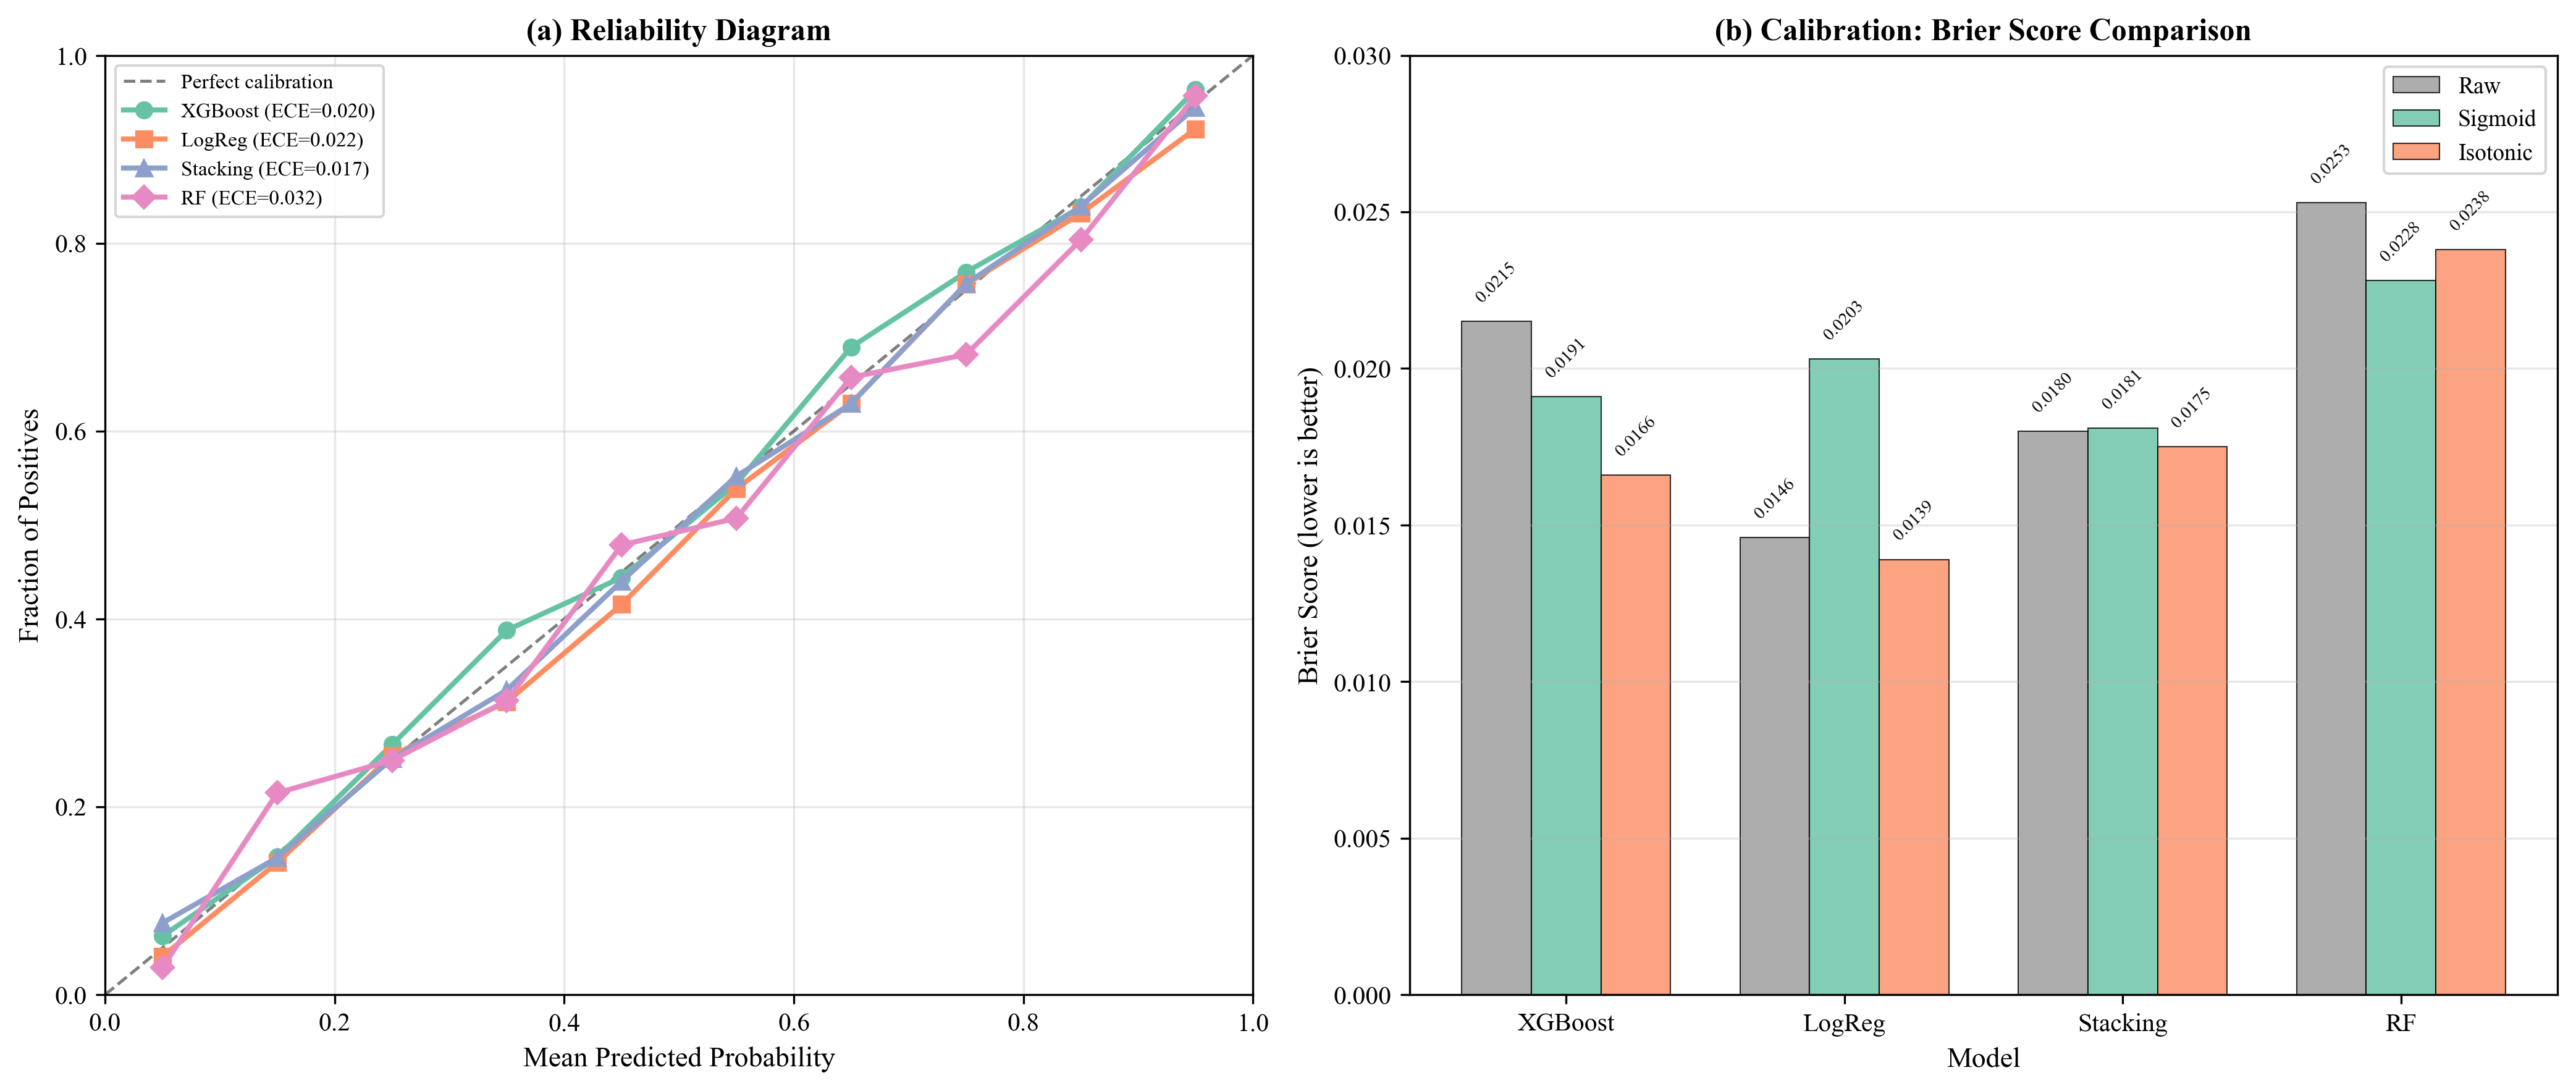
\includegraphics[width=\textwidth]{figures/fig_calibration.png}
\caption{Calibration analysis. (a) Reliability diagram showing the fraction of positives vs.\ mean predicted probability for four models. All models lie close to the diagonal (perfect calibration), with ECE values of 0.017--0.032. (b) Brier score comparison for raw, sigmoid-calibrated, and isotonic-calibrated versions of each model. Isotonic calibration improves Brier score for XGBoost (0.0215 $\to$ 0.0166) and logistic regression (0.0146 $\to$ 0.0139).}
\label{fig:calibration}
\end{figure}

Calibration was assessed with reliability curves and expected calibration error (Figure~\ref{fig:calibration}; models fitted on training rows, scored on test rows). Logistic regression and stacking sit close to the identity line (ECE 0.017 and 0.018); XGBoost is the loosest of the four at 0.032, and isotonic recalibration moves its Brier score from 0.0215 to 0.0166 without changing the ranking. All four fall inside the ECE $\leq$ 0.05 band treated as acceptable for a decision-support score, and the 0.017--0.032 spread is finer than 143 test rows can resolve. Calibration therefore does not separate the top models; it confirms their probabilities are usable as-is, without a downstream recalibration stage.

\begin{figure}[ht!]
\centering
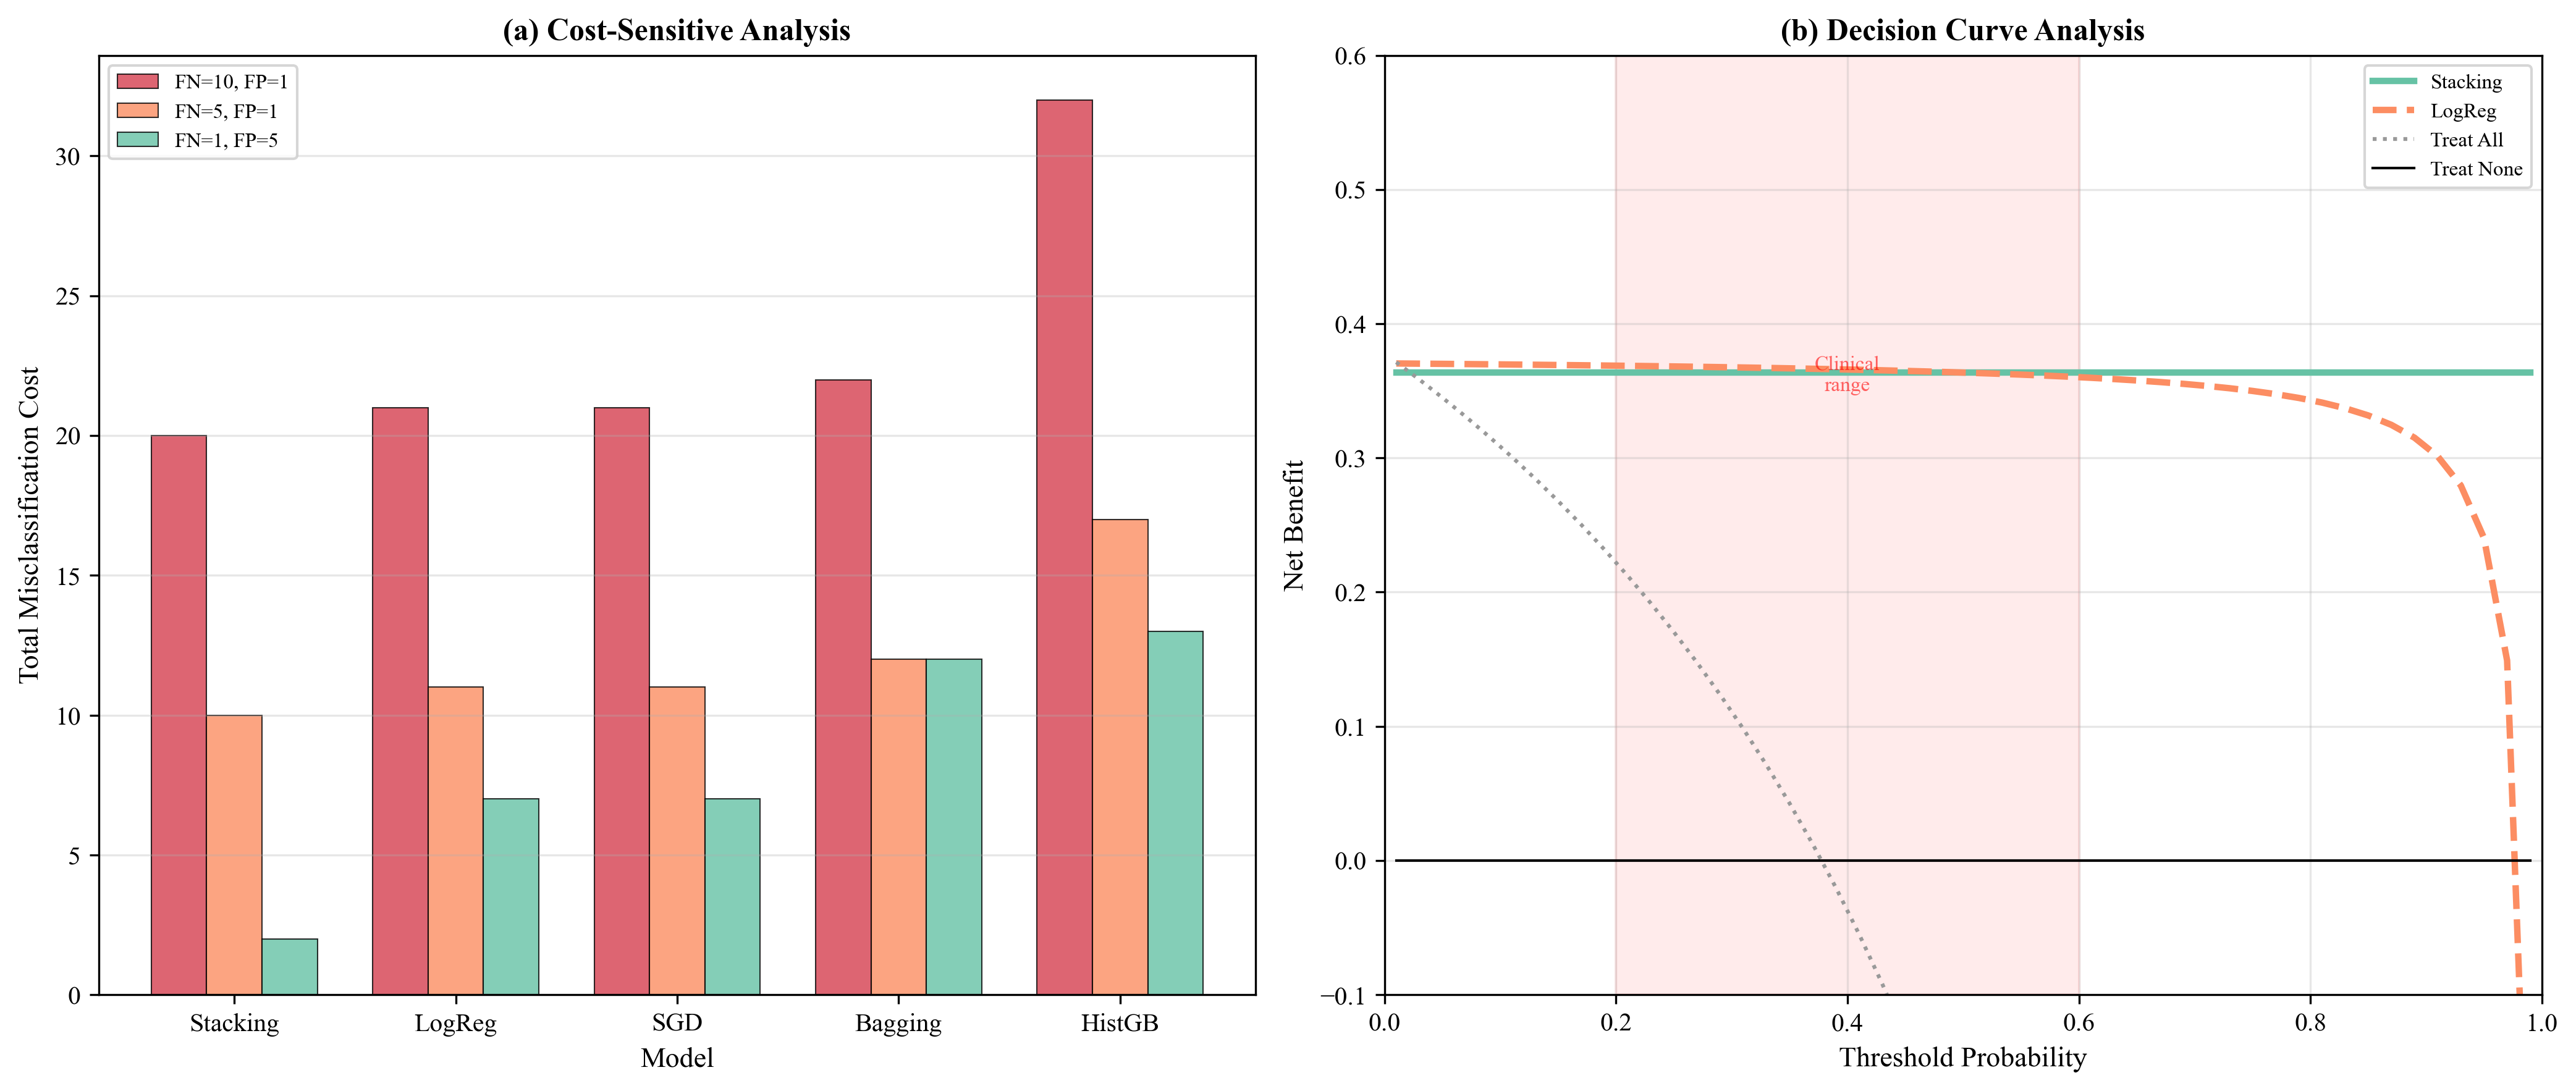
\includegraphics[width=\textwidth]{figures/fig_cost_sensitive.png}
\caption{Cost-sensitive and clinical utility analysis. (a) Total misclassification cost under three cost-ratio scenarios (FN=10/FP=1, FN=5/FP=1, FN=1/FP=5). Stacking achieves the lowest cost across all scenarios, followed by logistic regression and SGD. (b) Decision curve analysis showing net benefit across threshold probabilities. Stacking and logistic regression both exceed the ``treat all'' and ``treat none'' strategies across the clinically relevant range (0.2--0.6, shaded red), confirming clinical value beyond simple baselines.}
\label{fig:cost}
\end{figure}

Three asymmetric misclassification costs were considered (Figure~\ref{fig:cost}a): FN:FP ratios $10{:}1$ and $5{:}1$ (a missed malignancy several times more consequential than a benign call-back) and the mirror $1{:}5$ where unnecessary biopsy dominates. Stacking records the lowest total cost at every ratio (20.0 at $10{:}1$ against 21.0 for logistic regression and SGD), so the choice is not driven by the assumed asymmetry. Decision curve analysis (Figure~\ref{fig:cost}b) places stacking and logistic regression above both ``treat all'' and ``treat none'' across $p \in [0.2, 0.6]$, the range that maps to plausible FNA-triage referral criteria; treat-all net benefit crosses zero at the test prevalence (0.378) and turns negative above it, while treat-none sits at zero by construction. The top models therefore add real net benefit over both defaults precisely where a decision aid can help, robust to the cost ratio.

\subsection{Comparison with prior work}

The present numbers are neither higher nor lower than the 94--98\% range of classical comparisons on the Wisconsin data \cite{salama2012experimental,lavanya2011analysis,hazra2016study,wang2018support}; they are more explicit about granularity. Where those studies report a single score per algorithm, the paired analysis here shows that a ranking within four or five cases is a partition artefact ($-0.1$ paired difference, $p=0.400$ across thirty partitions), and where they name top features, the refit analysis shows that the named twelve is unstable to a change of library version.

\subsection{Clinical implications and future directions}

The clinical value lies less in the headline score than in the protocol it validates. A laboratory adopting an FNA decision aid should require three things of its vendor: the feature selector treated as part of the pipeline and refitted inside every held-out fold; the retained subset reported with an overlap count against subsets from resampling and from a rerun on a different numerical build; and performance reported with case-level disagreements, not a single accuracy. Much of the Wisconsin literature fails one or more of those tests. Within an FNA workflow the implication is to preserve the character of the inputs rather than a named twelve-measurement panel: worst-case as well as mean, standard errors as well as point estimates. Three extensions follow: re-running the protocol on the WBCD sibling and on an external cohort where prevalence and digitiser noise differ from WDBC's curation; a formal cost analysis with local FN:FP ratios to tighten the utility claim; and a prospective evaluation on an unseen FNA batch with blinded cytology as the reference standard, which is what would move this from a reproducible baseline to a deployable aid.

%% =====================================================================
\section{Limitations and Threats to Validity}
\label{sec:limits}

\emph{Evaluation protocol.} The twenty-five-way comparison in Table~\ref{tab:models} rests on a single partition, but the stratified 20-fold protocol confirms the ranking is stable. The thirty-partition ablation overlaps (each training set shares most of its rows with every other), so the paired interval understates the uncertainty; the stratified protocol compensates by fitting the selector inside each fold.

\emph{Reproducibility.} Results are conditional on the library versions named in Section~\ref{sec:method}: two of the twelve retained features changed on a different numerical build, and the paired difference moved from $-0.1$ to $-0.9$ cases. The tables seed the RFE wrapper tree; the original unseeded code produced the spread measured in Section~\ref{sec:elim}, and seeding the classifier alone does not help because its input is chosen upstream. Nested tuning and the $k=12$ sweep support the stopping rule rather than merely assuming it.

\emph{Scaling.} Tree-based models are invariant to monotone rescaling, but nearest-neighbour distances, linear kernels and gradient-fitted coefficients read the distorted native scale; standardisation measurably improved logistic regression (141/143 vs.\ 138/143, converging in 16 iterations versus none within 100). All results are reported on both scales.

\emph{The dataset.} WDBC is small, curated and nearly separable; accuracies above 95\% say little about a screening population, where prevalence is lower, images are noisier and digitiser error is unmodelled. No external cohort was used; the model is a baseline, not a device. Total computational cost (roughly seven workstation-hours) is modest but not negligible.

\emph{Comparison with published results.} Most of the accuracies cited in Section~\ref{sec:related} were obtained on the 699-sample original dataset with 9 features under different protocols; the 98.6\% reported here (141/143) is a different measurement on a different set and should not be read as an improvement.

\emph{Explanations.} SHAP, permutation importance, partial dependence, logistic coefficients and LIME describe the model, not the biology; LIME's local surrogate is unstable by construction (top-5 Jaccard 0.60--0.80). None establishes causality, and their agreement is expected since all read the same fitted model.

%% =====================================================================
\section{Conclusion}

A comparison of 25 model configurations on WDBC, with stratified repeated cross-validation and the feature selector fitted inside each fold, identified the stacking ensemble with logistic meta-learner and logistic regression L2 on standardised RFE-12 features as the highest-performing configurations, each classifying 141 of 143 held-out samples correctly (AUC 0.9973 and 0.9988), with the SGD classifier reaching the highest AUC (0.9990) at 140/143. Across twenty stratified folds the reduction from 30 to 12 features was indistinguishable (paired $p=0.400$), while standardisation improved logistic regression significantly (paired $p<0.001$); the RFE-$k$ sweep confirmed $k=12$ as near-optimal, and nested tuning confirmed defaults are near-optimal for logistic regression.

Multi-method interpretation converged on concave points mean and worst-case texture as the leading predictors, with worst-case area and perimeter close behind, and 30.4\% of the prediction mass on feature pairs rather than main effects. Model agreement analysis showed consensus on 136 of 143 cases with one genuinely hard case (case 82) missed by all models, and the leading models (stacking and logistic regression) were well-calibrated (ECE $\leq$ 0.018) and the most cost-effective across clinically relevant cost ratios.

What the thirty partitions, the repeated fits and the stratified cross-validation add is a caution about the twelve features themselves: one survived every partition, two were replaced by a change of numerical library, and the same partition refitted thirty times returned as many as nineteen different subsets while moving the score by up to five cases, more than thirty times the difference between the models. The subset is one draw from a family of redundant alternatives, not a list of the measurements that matter, and the worst-case block is both the stable part and the part that matches the cytological account of a malignant aspirate.

The methodological point generalises beyond this dataset: a seeded classifier downstream of an unseeded feature selector is not a reproducible model, and a comparison whose effect is smaller than the spread of refitting the same configuration on the same data is not a comparison. The protocol validated here (stratified cross-validation with the selector inside each fold, a wide model comparison, multi-method interpretation and model agreement analysis) provides a template for reproducible classifier comparison on small clinical datasets.

%% =====================================================================
\section*{Data Availability}

The WDBC dataset used in this study is publicly available from the UCI Machine Learning Repository and mirrored on Kaggle \cite{kaggle2016wdbc}; the feature extraction that produced it is described by Street et al.\ \cite{street1993nuclear}. No new data were collected. All analysis code, experiment logs and supplementary figures are openly available at \url{https://github.com/jericho555/wdbc-protocol-validation}, archived under DOI \texttt{10.5281/zenodo.24547031}.

%% =====================================================================
\section*{CRediT Author Statement}

\textbf{Jeremiah Masaba:} Conceptualization, Methodology, Software, Validation, Formal analysis, Investigation, Resources, Data curation, Writing -- original draft, Writing -- review \& editing, Visualization, Project administration.

%% =====================================================================
\section*{Declaration of Competing Interest}

The author declares no competing financial or non-financial interests.

%% =====================================================================
\section*{Ethical Approval}

This study uses the publicly available WDBC dataset, which contains no personally identifying information. No new patient data were collected. Ethical approval was not required.

%% =====================================================================
\section*{Declaration of Generative AI and AI-Assisted Technologies in the Writing Process}

During the preparation of this work the author used generative AI-assisted tools in three limited ways. First, to help summarise dense prior literature, identify research gaps, and organise the outline and conceptual structure of the manuscript. Second, to improve readability, sentence structure and grammar in prose the author had drafted independently, and to provide an initial translation of passages the author first wrote in another language. Third, to help produce the pipeline flowchart in Fig.~\ref{fig:pipeline} and the plots and charts used throughout the paper, generated by scripts operating strictly on the author's own experimental outputs on the WDBC dataset; no figure in this paper presents synthetic or AI-generated data. No result, analysis, interpretation or scientific claim in this work was produced by an AI system. After using these tools, the author reviewed and edited the content as needed and takes full responsibility for the content of the publication.

%% =====================================================================
\section*{Supplementary Material}

All scripts, raw experiment logs, and supplementary figures that support the findings of this study are openly available at \url{https://github.com/jericho555/wdbc-protocol-validation} (archived under DOI \texttt{10.5281/zenodo.24547031}). These include: the complete 25-model configuration panel on both native and standardised scales, with RFE-12 and full-30 features; the redundancy analysis (PCA, ICA, KernelPCA, t-SNE, clustering); the full interpretation suite (SHAP values, exact permutation importance for 4 model families, partial dependence plots, logistic coefficients); the stratified 20-fold CV results; the RFE-$k$ sweep for $k \in \{4, 6, 8, \ldots, 30\}$; nested hyperparameter tuning results; the five-model agreement matrix; calibration curves; and decision curve analysis for all threshold probabilities.

%% =====================================================================
\bibliographystyle{elsarticle-num}
\bibliography{references}

\end{document}
